\section{VECTƠ TRONG KHÔNG GIAN}
\subsection{LÝ THUYẾT CẦN NHỚ}
\subsubsection{Tổng của hai véc tơ}
\begin{enumerate}[\iconMT]
	\item \textbf{Định nghĩa:}
	 \immini{Trong không gian, cho hai véctơ $\vec{a}$ và $\vec{b}$. Lấy ba điểm $O$, $A$, $B$ sao cho $\vec{OA}=\vec{a}$, $\vec{AB}=\vec{b}$. Ta gọi $\vec{OB}$ là \textbf{tổng của hai véctơ} $\vec{a}$ và $\vec{b}$, ký hiệu $\vec{a}+\vec{b}$.\\
	 Phép lấy tổng của hai véctơ $\vec{a}$ và $\vec{b}$ được gọi là \textbf{phép cộng véctơ}.}
	 {
	 \begin{tikzpicture}[>=stealth,scale=.5,font=\footnotesize]
	 \foreach \x\y\t in {3/0.4/A1,4./4.4/A2,9.5/4.3/B1,14.5/1.3/B2,5/0/O}
	 \coordinate (\t) at (\x,\y);
	 \coordinate (A) at ($(A2)-(A1)+(O)$);
	 \coordinate (B) at ($(B2)-(B1)+(A)$);
	 \foreach \a/\b in {A1/A2,B1/B2,O/A,A/B,O/B}
	 {\draw[-{Stealth[length=2.5mm]}](\a)--(\b);}
	 \node at ($(A1)!1/2!(A2)$)[left=-2pt]{$\vec{a}$};
	 \node at ($(B1)!1/2!(B2)$)[above right=-2pt]{$\vec{b}$};
	 \node at ($(O)!1/2!(A)$)[left=-2pt]{$\vec{a}$};
	 \node at ($(A)!1/2!(B)$)[above right=-2pt]{$\vec{b}$};
	 \node at ($(O)!1/2!(B)$)[rotate=7,above=-2pt]{$\vec{a}+\vec{b}$};
	 \foreach \t/\g in {O/-140,A/90,B/0}
	 \draw[fill=black] (\t)circle(1.2pt) +(\g:12pt)node{$\t$};
	 \end{tikzpicture}}
	\item \textbf{Các quy tắc cần nhớ:}
	 \begin{listEX}[1]
	 \immini{\item [\ding{172}] Quy tắc ba điểm: Với ba điểm $A$, $B$, $C$, ta có
	 \fbox{$\vec{AB} + \vec{BC} = \vec{AC}$}
	 \item [\ding{173}] Quy tắc hình bình hành: Cho $ABCD$ là hình bình hành, ta có
	 \fbox{$\vec{AB} + \vec{AD} = \vec{AC}$}}{
	 \begin{tikzpicture}[scale=0.6, font=\footnotesize, line join=round, line cap=round]
	 \begin{scope}
	 \foreach \x\y\t in {0/0/A, -2/-2/B, 2.5/-1.5/C}
	 \coordinate (\t) at (\x,\y);
	 \foreach \a\b in {A/B, B/C,A/C}
	 \draw[-{Stealth[length=2mm]}] (\a)--(\b);
	 \foreach \t\g in {A/90, B/-100, C/-80}
	 \draw[fill=black] (\t)circle(0.6pt) +(\g:8pt)node{$\t$};
	 \end{scope}
	 \begin{scope}[xshift=5cm]
	 \foreach \x\y\t in {0/0/A, -1.5/-2/B, 2.5/-2/C,4/0/D}
	 \coordinate (\t) at (\x,\y);
	 \foreach \a\b in {A/B, A/D,A/C}
	 \draw[-{Stealth[length=2mm]}] (\a)--(\b);
	 \draw[dashed] (B)--(C)--(D);
	 \foreach \t\g in {A/90, B/-90, C/-45,D/50}
	 \draw[fill=black] (\t)circle(0.6pt) +(\g:8pt)node{$\t$};
	 \end{scope}
	 \end{tikzpicture}}
	 \immini{\item [\ding{174}] Quy tắc hình hộp:
	 Cho hình hộp $ABCD.A'B'C'D'$. Ta có
	 \fbox{$\vec{AB} + \vec{AD} + \vec{AA'} = \vec{AC'}$}
	 \begin{note}
	 Hệ thức tương tự: \quad $\vec{BA} + \vec{BC} + \vec{BB'} = \vec{BD'}$.
	 \end{note}
	 }{
	 \begin{tikzpicture}[scale=0.6, font=\footnotesize, line join=round, line cap=round]
	 \def\h{4}
	 \foreach \x\y\t in {0/0/A',-1/-1.1/B',2.6/-1.1/C'}
	 \coordinate (\t) at (\x,\y);
	 \coordinate (D') at ($(A')+(C')-(B')$);
	 \coordinate (A) at ($(A')+(0,2.5)$);
	 \coordinate (B) at ($(B')+(0,2.5)$);
	 \coordinate (C) at ($(C')+(0,2.5)$);
	 \coordinate (D) at ($(D')+(0,2.5)$);
	 \foreach \a\b in {A/B, A/D,A/C}
	 \draw[-{Stealth[length=2mm]}] (\a)--(\b);
	 \foreach \a\b in {A/A', A/C'}
	 \draw[-{Stealth[length=2mm]},dashed] (\a)--(\b);
	 \draw (D)--(C)--(B)--(B')--(C')--(D')--(D) (C')--(C);
	 \draw[dashed](B')--(A')--(D');
	 \foreach \t/\g in {A'/170,B'/-150,C'/-70,D'/0,A/100,B/170,C/-20,D/50}
	 \draw[fill=black] (\t) circle(1pt)
	 node[shift={(\g:7pt)}]{$\t$};
	 \end{tikzpicture}
	 }
	 \end{listEX}
	\item \textbf{Tính chất:}
	 \begin{itemize}
	 \item[\ding{172}] Tính chất giao hoán: $\vec{a}+\vec{b}=\vec{b}+\vec{a}$;
	 \item[\ding{173}] Tính chất kết hợp: $\left(\vec{a}+\vec{b}\right)+\vec{c}=\vec{a}+\left(\vec{b}+\vec{c}\right)$;
	 \item[\ding{174}] Với mọi véctơ $\vec{a}$, ta luôn có: $\vec{a}+\vec{0}=\vec{0}+\vec{a}=\vec{a}$.
	 \item[\ding{175}] Tổng của ba véctơ $\vec{a}$, $\vec{b}$, $\vec{c}$:\quad $\vec{a}+\vec{b}+\vec{c}=\left(\vec{a}+\vec{b}\right)+\vec{c}.$
	 \end{itemize}
\end{enumerate}
\subsubsection{Hiệu của hai véc tơ}
\begin{enumerate}[\iconMT]
	\item \textbf{Véctơ đối:}
	 \begin{listEX}[1]
	 \item [\ding{172}] Vectơ đối của $\vec{a}$ kí hiệu là $-\vec{a}$.
	 \item [\ding{173}] Vectơ đối của $\vec{AB}$ là $\vec{BA}$: $-\vec{AB}=\vec{BA}$.
	 \item [\ding{174}] Vectơ $\vec{0}$ được coi là vectơ đối của chính nó.
	 \end{listEX}
	 \immini{
	\item \textbf{Định nghĩa hiệu của hai véctơ:} Trong không gian, cho hai véctơ $\vec{a}$, $\vec{b}$. Ta gọi $\vec{a}+\left(-\vec{b}\right)$ là \textbf{hiệu của hai véctơ} $\vec{a}$ và $\vec{b}$, ký hiệu $\vec{a}-\vec{b}$.\\
	 Phép lấy hiệu của hai véctơ được gọi là \textbf{phép trừ véctơ}.
	\item \textbf{Các quy tắc cần nhớ:}
	 \begin{listEX}[1]
	 \item [\ding{172}] Với ba điểm $A$, $B$, $C$ ta có $\vec{AB}-\vec{AC}=\vec{CB}$.
	 \item [\ding{173}] Hai véc tơ $\vec{a}$ và $\vec{b}$ đối nhau thì $\vec{a}+\vec{b}=\vec{0}$.
	 \end{listEX}
	 }{
	 \begin{tikzpicture}[scale=1, font=\footnotesize, line join=round, line cap=round]
	 \foreach \x\y\t in {0/0/O,1.5/1/A,3.1/-0.4/B,-0.3/1/a1,1.1/1.6/b1}
	 \coordinate (\t) at (\x,\y);
	 \coordinate (a2) at ($(a1)+(A)$);
	 \coordinate (b2) at ($(b1)+(B)$);
	 \foreach \a\b in {a1/a2, b1/b2,O/A,O/B,B/A}
	 \draw[-{Stealth[length=2mm]}] (\a)--(\b);
	 \path (a1)--(a2)node[pos=0.5,above left]{$\vec{a}$}
	 (b1)--(b2)node[pos=0.5,above]{$\vec{b}$}
	 (O)--(A)node[pos=0.5,above left]{$\vec{a}$}
	 (O)--(B)node[pos=0.5,below]{$\vec{b}$}
	 (B)--(A)node[pos=0.7,right=3pt]{$\vec{a}-\vec{b}$};
	 \foreach \t\g in {A/90, O/180, B/0}
	 \draw[fill=black] (\t)circle(0.2pt) +(\g:5pt)node{$\t$};
	 \end{tikzpicture}}
\end{enumerate}
\subsubsection{Tích của một số với một véc-tơ}
\begin{enumerate}[\iconMT]
	\item \textbf{Định nghĩa:} Cho số thực $k\ne 0$ và vectơ $\vec{a} \ne \vec{0}$. Tích của một số $k$ với vectơ $\vec{a}$ là một vectơ, kí hiệu là $k\vec{a}$, được xác định như sau:
	 \begin{itemize}
	 \item Cùng hướng với vectơ $\vec{a}$ nếu $k>0$, ngược hướng với vectơ $\vec{a}$ nếu $k<0$.
	 \item Có độ dài bằng $|k| \cdot |\vec{a}|$.
	 \end{itemize}
	 \begin{note}
	 $0\cdot \vec{a}=\vec{0}$ và $k\cdot \vec{0}=\vec{0}$.
	 \end{note}
	 % \immini{\textbf{Ví dụ:} Theo hình vẽ bên, thì $\vec{b}=3\vec{a}$; $\vec{c}=-2\vec{a}$; $\vec{c}=-\dfrac{2}{3}\vec{b}$.
	 % }{
	 % \begin{tikzpicture}[>=stealth,scale=0.5, line join=round, line cap=round]
	 % 	 \draw[line width=0.05pt,gray,dashed] (-0.7,-0.7) grid (8.7,3.7);
	 % 	 \draw[->,thick](1,2)--(2,3)node[above left]{$\vec{a}$};
	 % 	 \draw[->,thick](1,0)--(4,3)node[above right]{$\vec{b}$};
	 % 	 \draw[->,thick](7,3)--(5,1)node[below right]{$\vec{c}$};
	 % \end{tikzpicture}}
	\item \textbf{Hệ thức trung điểm, trọng tâm:}
	 \immini{
	 \begin{itemize}
	 \item [\ding{172}] $I$ là trung điểm của đoạn thẳng $AB$ thì
	 \begin{itemize}
	 \item [$\bullet$] $\vec{IA} + \vec{IB} = \vec 0$;
	 \item [$\bullet$] $\vec{IA}=-\vec{IB}$; $\vec{AI}=\dfrac{1}{2}\vec{AB}$;...
	 \end{itemize}
	 \item [\ding{173}] $G$ là trọng tâm của tam giác $ABC$ thì
	 \begin{listEX}[1]
	 \item [$\bullet$] $\vec{GA}+\vec{GB}+\vec{GC}=\vec{0}$;
	 \item [$\bullet$] $\vec{GA}=-\dfrac{2}{3}\vec{AK}$; $\vec{GA}=-2\vec{GK}$;...
	 \end{listEX}
	 \end{itemize}}{
	 \begin{tikzpicture}[scale=0.8, font=\footnotesize, line join=round, line cap=round]
	 \begin{scope}
	 \foreach \x\y\t in {-2/-2/A, 0/0/B}
	 \coordinate (\t) at (\x,\y);
	 \coordinate (I) at ($(A)!0.5!(B)$);
	 \foreach \a\b in {A/B}
	 \draw[] (\a)--(\b);
	 \foreach \t\g in {A/-90, B/40,I/1200}
	 \draw[fill=black] (\t)circle(0.6pt) +(\g:8pt)node{$\t$};
	 \end{scope}
	 \begin{scope}[xshift=4cm]
	 \foreach \x\y\t in {0/0/A, -2/-2/B, 2.5/-2/C}
	 \coordinate (\t) at (\x,\y);
	 \coordinate (M) at ($(A)!0.5!(B)$);
	 \coordinate (N) at ($(A)!0.5!(C)$);
	 \coordinate (K) at ($(C)!0.5!(B)$);
	 \coordinate (G) at ($(A)!2/3!(K)$);
	 \foreach \a\b in {A/B, B/C, A/C, A/K, M/C, B/N}
	 \draw[] (\a)--(\b);
	 \foreach \t\g in {A/90, B/-100, C/-80, M/120, N/40, K/-90,G/60}
	 \draw[fill=black] (\t)circle(0.8pt) +(\g:10pt)node{$\t$};
	 \end{scope}
	 \end{tikzpicture}}
	\item \textbf{Nhận xét:}
	 \begin{itemize}
	 \item[\ding{172}] Với hai véctơ $\vec{a}$ và $\vec{b}$ bất kỳ, với mọi số $h$ và $k$, ta luôn có
	 \begin{enumEX}[$\bullet$]{3}
	 \item $k\left(\vec{a}+\vec{b}\right)=k\vec{a}+k\vec{b}$;
	 \item $\left(h+k\right)\vec{a}=h\vec{a}+k\vec{a}$;
	 \item $h\left(k\vec{a}\right)=\left(hk\right)\vec{a}$;
	 \item $1\cdot \vec{a}=\vec{a}$;
	 \item $\left(-1\right)\cdot\vec{a}=-\vec{a}$;
	 \item $k\vec{a}=\vec{0} \Leftrightarrow \hoac{&\vec{a}=\vec{0}\\& k=0}$.
	 \end{enumEX}
	 \item[\ding{173}] Hai véctơ $\vec{a}$ và $\vec{b}$ ($\vec{b}$ khác $\vec{0}$) cùng phương khi và chỉ khi có số $k$ sao cho $\vec{a}=k\vec{b}$.
	 \item[\ding{174}] Ba điểm phân biệt $A$, $B$, $C$ thẳng hàng khi và chỉ khi có số $k \neq 0$ để $\vec{AB}=k\vec{AC}$.
	 \end{itemize}
\end{enumerate}
\subsubsection{Tích vô hướng của hai véc-tơ}
\begin{enumerate}[\iconMT]
	\item \textbf{Góc giữa hai véctơ:}
	 \immini{
	 Trong không gian, cho $\vec{u}$ và $\vec{v}$ là hai véctơ khác $\vec{0}$. Lấy một điểm $A$ bất kỳ, gọi $B$ và $C$ là hai điểm sao cho $\vec{AB}=\vec{u}$, $\vec{AC}=\vec{v}$. Khi đó, ta gọi $\widehat{BAC}$ là góc giữa hai véctơ $\vec{u}$ và $\vec{v}$, ký hiệu $\left(\vec{u}, \vec{v}\right)$.
	 \begin{note}
	 $0^{\circ} \leq \left(\vec{u},\vec{v}\right) \leq 180^{\circ}$.
	 \end{note}
	 \begin{note}
	 \begin{itemize}
	 \item [$\bullet$] Nếu $\vec{u}$ cùng hướng với $\vec{v}$ thì $\left(\vec{u}, \vec{v}\right)=0^\circ$;
	 \item [$\bullet$] Nếu $\vec{u}$ ngược hướng với $\vec{v}$ thì $\left(\vec{u}, \vec{v}\right)=180^\circ$;
	 \item [$\bullet$] Nếu $\vec{u}$ vuông góc với $\vec{v}$ thì $\left(\vec{u}, \vec{v}\right)=90^\circ$.
	 \end{itemize}
	 \end{note}
	 }{\vspace{-0.5cm}
	 \begin{tikzpicture}[scale=0.8, font=\footnotesize, line join=round, line cap=round]
	 \foreach \x\y\t in {0/0/A,2/0.8/B,3.2/-1./C,-1/1/u1,-0.5/-1.5/v1}
	 \coordinate (\t) at (\x,\y);
	 \coordinate (u2) at ($(u1)+(B)$);
	 \coordinate (v2) at ($(v1)+(C)$);
	 \draw (-1.5,-1.2)--(3.5,-1.2)--(4.5,1)--(-0.5,1)--cycle;
	 \draw[dashed] (A)--(u1) (B)--(u2) (A)--(v1) (C)--(v2);
	 \foreach \a\b in {A/B, A/C,u1/u2,v1/v2}
	 \draw[-{Stealth[length=2mm]}] (\a)--(\b);
	 \foreach \t\g in {A/-170, B/0, C/50}
	 \draw[fill=black] (\t)circle(0.6pt) +(\g:8pt)node{$\t$};
	 \path (A) pic[draw,angle radius=9]{angle=C--A--B};
	 \path
	 (u1)--(u2)node[pos=0.5,above]{$\vec{u}$}
	 (v1)--(v2)node[pos=0.5,above]{$\vec{v}$};
	 \end{tikzpicture}}
	\item \textbf{Định nghĩa tích vô hướng của hai véc tơ:}
	 Trong không gian, cho hai véctơ $\vec{u}$ và $\vec{v}$ khác $\vec{0}$.\\
	 Tích vô hướng của hai véctơ $\vec{u}$ và $\vec{v}$ là một số, kí hiệu $\vec{u} \cdot \vec{v}$, được xác định bởi công thức
	 \fbox{$\vec{u} \cdot \vec{v}=|\vec{u}| \cdot |\vec{v}| \cdot \cos (\vec{u}, \vec{v})$}
	 \vspace{-0.6cm}
	 \begin{note}
	 \begin{itemize}
	 \item[\ding{172}] Trong trường hợp $\vec{u}=0$ hoặc $\vec{v}=0$, ta quy ước $\vec{u} \cdot \vec{v}=0$.
	 \item[\ding{173}] $\vec{u} \cdot \vec{u}=\vec{u}^2=|\vec{u}|^2$; \quad $\vec{u}^2 \geqslant 0$. $ \vec{u}^2 = 0 \Leftrightarrow \vec{u}=\vec{0}$.
	 \item[\ding{174}] Với hai véctơ $\vec{u}$, $\vec{v}$ khác $\vec{0}$, ta có $\cos (\vec{u},\vec{v}) = \dfrac{\vec{u} \cdot \vec{v}}{|\vec{u}| \cdot |\vec{v}|}$
	 \item[\ding{175}] Với hai véctơ $\vec{u}$, $\vec{v}$ khác $\vec{0}$, ta có $\vec{u} \perp \vec{v} \Leftrightarrow \vec{u} \cdot \vec{v}= \vec{0}$.
	 \end{itemize}
	 \end{note}
	\item \textbf{TÍnh chất:} Với ba véctơ $\vec{a}$, $\vec{b}$, $\vec{c}$ và số thực $k$, ta có:
	 \begin{enumEX}[$\bullet$]{3}
	 \item $\vec{a} \cdot \vec{b}= \vec{b} \cdot \vec{a}$;
	 \item $\vec{a} \cdot \left( {\vec{b} + \vec{c}} \right) = \vec{a} \cdot \vec{b} + \vec{a} \cdot \vec{c}$;
	 \item $(k\vec{a}) \cdot \vec{b}= k(\vec{a} \cdot \vec{b}) = \vec{a} \cdot (k\vec{b})$.
	 \end{enumEX}
\end{enumerate}
\subsection{PHÂN LOẠI VÀ PHƯƠNG PHÁP GIẢI TOÁN}
\begin{dang}{Xác định véc-tơ, chứng minh đẳng thức véc tơ,độ dài véc tơ}
\end{dang}
\boxmini{BÀI TẬP TỰ LUẬN}
\setcounter{vd}{0}
\begin{vd}
	\immini{Cho hình hộp $ABCD.A'B'C'D'$. Hãy xác định các véc-tơ (khác $\vec{0}$) có điểm đầu, điểm cuối là các đỉnh của hình hộp $ABCD.A'B'C'D'$ thỏa
	\begin{tasks}(2)
	\task cùng phương với $\vec{AB}$;
	\task cùng phương $\vec{AA'}$;
	\task bằng với $\vec{AD}$;
	\task bằng với $\vec{A'B}$;
	\task đối với $\vec{CD'}$;
	\task đối với $\vec{B'C}$.
	\end{tasks}}{
	\begin{tikzpicture}[scale=0.7, font=\footnotesize,>=stealth]
	%Gán số liệu.
	\def\canhAD{3};\def\canhBA{2};\def\gocBAD{-130};\def\h{3};\def\xdinhA'{-0.5};
	%Gán tọa độ.
	\coordinate (A) at (0,0);
	\coordinate (B) at ($(A)+(\gocBAD:\canhBA)$);
	\coordinate (C) at ($(B)+(0:\canhAD)$);
	\coordinate (D) at ($(A)+(0:\canhAD)$);
	\coordinate (A') at ($(A)+(\xdinhA',\h)$);
	\coordinate (B') at ($(B)+(\xdinhA',\h)$);
	\coordinate (C') at ($(C)+(\xdinhA',\h)$);
	\coordinate (D') at ($(D)+(\xdinhA',\h)$);
	%Vẽ khối lẳng trụ ABCD.A'B'C'D'.
	\draw (A')--(B')--(B)--(C)--(C')--(D')--cycle (B')--(C') (D')--(D)--(C);
	\draw[dashed] (A)--(D) ;
	\draw[->,dashed] (A)--(C');
	\draw[->,dashed] (A)--(A');
	\draw[->, dashed] (A)--(D);
	\draw[->, dashed] (A)--(B);
	\draw[->, dashed] (A)--(C);
	%Gán nhãn.
	\foreach \x/\y in {A/180, B/180, C/0, D/0, A'/180, B'/180, C'/0, D'/0}{\fill (\x) circle(1pt) ($(\x)+(\y:0.3cm)$) node{$\x$};}
	\end{tikzpicture}}
\end{vd}
\dongcham{3}
\begin{vd}
	Cho hình chóp $S . A B C D$ có đáy $A B C D$ là hình bình hành. Gọi $M$, $N$, $O$ lần lượt là trung điểm của $A B, C D$ và $AC$. Chứng minh rằng
	\begin{listEX}[3]
	\item $\vec{B N}$ và $\vec{D M}$ đối nhau;
	\item $\vec{SA}+\vec{SB}+\vec{SC}+\vec{SD}=4\vec{SO}$;
	\item $\vec{S D}-\vec{B N}-\vec{C M}=\vec{S C}$.
	\end{listEX}
	\loigiai{
	\immini{\vspace*{-3mm}
	\begin{enumerate}
	\item Tứ giác $A B C D$ là hình bình hành nên $A B=C D$ và $A B\parallel C D$, suy ra $B M=DN$ và $B M \parallel D N$.\\
	 Do đó $BMDN$ là hình bình hành.\\
	 Hai véc-tơ $\vec{BN}$ và $\vec{DN}$ có cùng độ dài và ngược hướng nên chúng là hai véc-tơ đối nhau.
	\item Ta có $\vec{SA}+\vec{SC}=2\vec{SO}$; $\vec{SB}+\vec{SD}=2\vec{SO}$. Suy ra
	 $$\vec{SA}+\vec{SB}+\vec{SC}+\vec{SD}=4\vec{SO}.$$
	\item Từ câu a, ta có $\vec{BN}=-\vec{DM}$.\\
	 Suy ra $\vec{S D}-\vec{B N}-\vec{C M}=\vec{S D}+\vec{DM}-\vec{CM}=\vec{SM}+\vec{MC}=\vec{S C}$.
	\end{enumerate}
	}{
	\begin{tikzpicture}[line join=round, line cap = round, >=stealth, scale=.9,font=\footnotesize]
	\def\a{4}
	\path 	(0:0) coordinate (A)
	++(0:\a) coordinate (D)
	++(-130:\a/2) coordinate (C)
	($(A)+(C)-(D)$) coordinate (B)
	($(A)+(80:0.7*\a)$) coordinate (S)
	(intersection of A--C and B--D) coordinate (O)
	($(A)!0.5!(B)$) coordinate (M)
	($(C)!0.5!(D)$) coordinate (N)
	($(A)!0.5!(C)$) coordinate (O)
	;%giao điểm O
	\draw[dashed] 	(B)--(A)--(D)	(A)--(S) (A)--(C) (B)--(D);
	\draw 	(B)-- (C)--(D)
	(B)--(S)	(C)--(S)	(D)--(S);
	\foreach \x/\g in {A/135,B/-135,C/-45,D/45,S/90,M/-50,N/-30,O/-90}
	\fill[black] 	(\x) circle (1pt)
	($(\g:3mm)+(\x)$) node {$\x$};
	\draw [dashed] (D)--(M) (B)--(N);
	\end{tikzpicture}}
	}
\end{vd}
\dongcham{16}
\begin{vd}
	Cho hình lập phương $A B C D . A' B' C' D'$ cạnh bằng $a$. Gọi $G$ là trọng tâm tam giác $AB'D'$.
	\begin{tasks}(2)
	\task Tìm vectơ: $\vec{C C'}+\vec{B A}$; \quad $\vec{C C'}+\vec{B A}+\vec{D' A'}$.
	\task Chứng minh: $\vec{B C}+\vec{D C}+\vec{A A'}=\vec{A C'}$.
	\task Chứng minh: $\vec{B'B} + \vec{AD} + \vec{CD} = \vec{B'D}$.
	\task Chứng minh: $\vec{BB'} - \vec{C'B'} - \vec{D'C'} = \vec{BD'}$.
	\task Chứng minh: $\vec{A'C} = 3\vec{A'G}$.
	\task Tính độ dài véc tơ $\vec{u}= \vec{AB}+\vec{A'D'}+\vec{AA'}$.
	\end{tasks}
	\loigiai{
	\begin{enumerate}[a)]
	\immini{
	\item Vì $A B C D . A' B' C' D'$ là hình hộp nên $\vec{B A}=\vec{C D}$ và $\vec{D' A'}=\vec{C B}$.\\
	 Suy ra $\vec{C C'}+\vec{B A}+\vec{D' A'}=\vec{C C'}+\vec{C D}+\vec{C B}=\vec{C A'}$.
	\item Vì tứ giác $A B C D$ là hình bình hành nên $\vec{B C}=\vec{A D}$ và $\vec{D C}=\vec{A B}$. Áp dụng quy tắc hình hộp suy ra $$\vec{B C}+\vec{D C}+\vec{A A'}=\vec{A D}+\vec{A B}+\vec{A A'}=\vec{A C'}$$
	\item Ta có $\vec{AD} = \vec{B'C'}$, $\vec{CD} = \vec{B'A'}$. Do đó
	 $$\vec{B'B} + \vec{AD} + \vec{CD} = \vec{B'B} + \vec{B'C'} + \vec{B'A'} = \vec{B'D}.$$
	\item Ta có \begin{eqnarray*}
	 \vec{BB'} - \vec{C'B'} - \vec{D'C'} &=& \vec{BB'} - \left( \vec{D'C'} + \vec{C'B'} \right)
	 = \vec{BB'} - \vec{D'B'} \\
	 &=& \vec{BB'} + \left( - \vec{D'B'}\right)
	 = \vec{BB'} + \vec{B'D'}= \vec{BD'}.
	 \end{eqnarray*}
	 }{
	 \begin{tikzpicture}[scale=0.8, font=\footnotesize, line join=round, line cap=round]
	 \def\h{4}
	 \foreach \x\y\t in {0/0/A,-1/-1.1/B,2.6/-1.1/C}
	 \coordinate (\t) at (\x,\y);
	 \coordinate (D) at ($(A)+(C)-(B)$);
	 \coordinate (A') at ($(A)+(0,3.2)$);
	 \coordinate (B') at ($(B)+(0,3.2)$);
	 \coordinate (C') at ($(C)+(0,3.2)$);
	 \coordinate (D') at ($(D)+(0,3.2)$);
	 \draw (B')--(A')--(D')--(C')--(B')--(B)--(C)--(D)--(D') (C')--(C);
	 \draw[dashed](B)--(A)--(D) (A)--(A');
	 \foreach \t/\g in {A/170,B/-150,C/-70,D/0,A'/100,B'/170,C'/-20,D'/50}
	 \draw[fill=black] (\t) circle(1pt)
	 node[shift={(\g:7pt)}]{$\t$};
	 \end{tikzpicture}
	 }
	\item Do $G$ là trọng tâm tam giác $AB'D'$ nên $\vec{GA} + \vec{GB'} + \vec{GD'} = \vec{0}$. Khi đó, theo quy tắc hình hộp ta có
	 \begin{eqnarray*}
	 & \vec{A'C} & = \vec{A'A} + \vec{A'B'} + \vec{A'D'}\\
	 & & = \vec{A'G} + \vec{GA} + \vec{A'G} + \vec{GB'} + \vec{A'G} + \vec{GD'}\\
	 & & = 3\vec{A'G}.
	 \end{eqnarray*}
	\item Ta có $\vec{u}= \vec{AB}+\vec{A'D'}+\vec{AA'}=\vec{AB}+\vec{AD}+\vec{AA'}=\vec{AC'}$. Suy ra
	 $\big|\vec{u}\big|=AC'=a\sqrt{3}.$
	\end{enumerate}
	}
\end{vd}
\dongcham{34}
\begin{vd}%[2H2H1-4]
	\immini{
	Ba lực $\vec{F_1}$, $\vec{F_2}$, $\vec{F_3}$ cùng tác động vào một vật có phương đôi một vuông góc nhau và có độ lớn lần lượt là $2 \mathrm{\,N}$, $3 \mathrm{\,N}$, $4 \mathrm{\,N}$.
	\begin{tasks}
	\task Tính độ lớn hợp lực của $\vec{F_2}$, $\vec{F_3}$.
	\task Tính độ lớn hợp lực của ba lực đã cho.
	\end{tasks}}
	{
	\begin{tikzpicture}[scale=1.3, font=\footnotesize, line join=round, line cap=round]
	\foreach \x\y\t in {0/0/O,0/1/a,1.3/0/b,-1.2/-1/c}
	\coordinate (\t) at (\x,\y);
	\foreach \a\b in {O/a,O/b,O/c}
	\draw[-{Stealth[length=2mm]}] (\a)--(\b);
	\path (O)--(a) node[pos=0.5,left]{$\vec{F_1}$}
	(O)--(b) node[pos=0.5,above]{$\vec{F_2}$}
	(O)--(c) node[pos=0.5,above left]{$\vec{F_3}$};
	\path
	pic[draw,angle radius=4]{right angle=a--O--b}
	pic[draw,angle radius=4]{right angle=c--O--b}
	pic[draw,angle radius=4]{right angle=c--O--a};
	\end{tikzpicture}}
	\loigiai{
	\immini{
	\begin{enumerate}[a)]
	\item Gọi $O$ là vị trí trên vật mà ba lực cùng tác động vào. Gọi$A$, $B$, $C$ là các điểm sao cho $\vec{F_1}=\vec{OA}$, $\vec{F_2}=\vec{OB}$, $\vec{F_3}=\vec{OC}$. Khi đó
	 $$\left|\vec{F_2}+\vec{F_3}\right|=OE=\sqrt{3^2+4^2}=5 \text{N}.$$
	\item Dựng các hình chữ nhật $OBEC$ và $OEFA$ thì ta có
	 $$\heva{&\vec{OB}+\vec{OC}=\vec{OE}\\&\vec{OA}+\vec{OE}=\vec{OF}.}$$
	 Do đó $\vec{F_1}+\vec{F_2}+\vec{F_3}=\vec{OA}+\vec{OB}+\vec{OC}=\vec{OA}+\vec{OE}=\vec{OF}.$\\
	 Vậy độ lớn hợp lực của $F_1$, $\vec{F_2}$ và $\vec{F_3}$ là
	 $$\begin{aligned}
	 \left|\vec{F_1}+\vec{F_2}+\vec{F_3}\right|=OF
	 & =\sqrt{OA^2+OE^2} \\
	 & =\sqrt{OA^2+OB^2+OC^2} \\
	 & =\sqrt{2^2+3^2+4^2}=\sqrt{29} \mathrm{\,N}.
	 \end{aligned}$$
	\end{enumerate}
	}
	{
	\begin{tikzpicture}[scale=1.8, font=\footnotesize, line join=round, line cap=round]
	\foreach \x\y\t in {0/0/O,0/1/A,1.3/0/B,-0.9/-1.2/C}
	\coordinate (\t) at (\x,\y);
	\coordinate (E) at ($(B)+(C)$);
	\coordinate (F) at ($(A)+(E)$);
	\foreach \a\b in {O/A,O/B,O/C,O/F,O/E}
	\draw[-{Stealth[length=2mm]}] (\a)--(\b);
	\path
	(O)--(A) node[pos=0.5,left]{$\vec{F_1}$}
	(O)--(B) node[pos=0.5,above]{$\vec{F_2}$}
	(O)--(C) node[pos=0.5,above left]{$\vec{F_3}$};
	\path
	pic[draw,angle radius=4]{right angle=A--O--B}
	pic[draw,angle radius=4]{right angle=C--O--B}
	pic[draw,angle radius=4]{right angle=C--O--A};
	\foreach \t\g in {A/90, B/0, C/180,E/-80,F/0,O/180}
	\draw[fill=black] (\t)circle(0.1pt) +(\g:4pt)node{$\t$};
	\draw[dashed] (C)--(E)--(B) (A)--(F)--(E);
	\end{tikzpicture}}
	}
\end{vd}
\dongcham{23}
\boxmini{BÀI TẬP TRẮC NGHIỆM}
\textbf{PHẦN I.} \textit{Câu trắc nghiệm nhiều phương án lựa chọn. Mỗi câu hỏi học sinh chỉ chọn một phương án.}\\
\setcounter{ex}{0}
\Opensolutionfile{ans}[ans/2H2-B1-d1-1]
%%==========Câu 1
\begin{ex}%[1H3B1-1]
	\immini{Cho hình hộp $ABCD.EFGH$. Các véc-tơ có điểm đầu và điểm cuối là các đỉnh của hình hộp và bằng véc-tơ $\vec{AB}$ là các véc-tơ nào sau đây?
	\choice
	{$\vec{CD}$, $\vec{HG}$, $\vec{EF}$}
	{\True $\vec{DC}$, $\vec{HG}$, $\vec{EF}$}
	{$\vec{DC}$, $\vec{HG}$, $\vec{FE}$}
	{$\vec{DC}$, $\vec{GH}$, $\vec{EF}$}}{
	\begin{tikzpicture}[scale=0.75, font=\footnotesize, line join=round, line cap=round]
	\foreach \x\y\t in {0/0/A,-0.8/-1.1/B,2.8/-1.1/C}
	\coordinate (\t) at (\x,\y);
	\coordinate (D) at ($(A)+(C)-(B)$);
	\coordinate (E) at ($(A)+(-0.5,2.5)$);
	\coordinate (F) at ($(B)+(E)-(A)$);
	\coordinate (G) at ($(C)+(E)-(A)$);
	\coordinate (H) at ($(D)+(E)-(A)$);
	\foreach \a\b in {A/B, A/D,A/E}
	\draw[dashed] (\a)--(\b);
	\foreach \a\b in {C/D,C/B,C/G}
	\draw[] (\a)--(\b);
	\draw (F)--(E)--(H)--(G)--(F)--(B) (D)--(H);
	\foreach \t/\g in {A/170,B/-130,C/-60,D/0,E/90,F/180,G/-20,H/70}
	\draw[fill=black] (\t) circle(1pt)
	node[shift={(\g:7pt)}]{$\t$};
	\end{tikzpicture}}
	\loigiai{
	Các véc-tơ bằng với véc-tơ $\vec{AB}$ là $\vec{DC}$, $\vec{HG}$, $\vec{EF}$
	}
\end{ex} \dongcham{2}
%%==========Câu 2
\begin{ex}%[1H3B1-2]
	\immini{Cho hình hộp $ABCD.A'B'C'D'.$ Trong các khẳng định sau, khẳng định nào \textbf{sai}?
	\choice
	{$\vec{AB}+\vec{B'D'}=\vec{AD}$}
	{$\vec{AB}+\vec{CD}=\vec{0}$}
	{$\vec{AC'}+\vec{A'C}=2\vec{AC}$}
	{\True $\vec{AC}-\vec{D'D}=\vec{0}$}}{
	\begin{tikzpicture}[scale=0.55, font=\footnotesize, line join=round, line cap=round]
	\foreach \x\y\t in {0/0/A,-2/-1.5/B,3.9/0/D,-0.5/3.5/A'}
	\coordinate (\t) at (\x,\y);
	\coordinate (C) at ($(B)+(D)-(A)$);
	\coordinate (B') at ($(A')+(B)-(A)$);
	\coordinate (C') at ($(B')+(C)-(B)$);
	\coordinate (D') at ($(C')+(D)-(C)$);
	\draw (A')--(B')--(B)--(C)--(C');
	\draw (A')--(D')--(D);
	\draw (D')--(C') (C)--(D);
	\draw (B')--(C') (D)--(D');
	\draw[dashed] (A)--(B) (A')--(A)--(D);
	\foreach \t/\g in {A/180,B/180,C/0,D/0,A'/180,B'/180,C'/0,D'/0} \draw (\t) node[shift={(\g:10pt)}]{$\t$};
	\end{tikzpicture}}
	\loigiai{
	\immini{
	\begin{itemize}
	\item [$\bullet$] $\vec{AB}+\vec{B'D'}=\vec{AB}+\vec{BD}=\vec{AD}$'
	\item [$\bullet$] $\vec{AB}$ và $\vec{CD}$ đối nhau nên $\vec{AB}+\vec{CD}=\vec{0}$.
	\item [$\bullet$] Theo quy tắc hình bình hành ta có\\ $\vec{AC'}+\vec{A'C}=\vec{AC}+\vec{AA'}+\vec{A'A}+\vec{A'C'}=2\cdot\vec{AC}.$
	\item [$\bullet$] $\vec{AC}-\vec{D'D}=\vec{AC}+\vec{CC'}=\vec{AC'}$
	\end{itemize}
	}
	{\begin{tikzpicture}[scale=0.55, font=\footnotesize, line join=round, line cap=round]
	\foreach \x\y\t in {0/0/A,-2/-1.5/B,3.9/0/D,-0.5/3.5/A'}
	\coordinate (\t) at (\x,\y);
	\coordinate (C) at ($(B)+(D)-(A)$);
	\coordinate (B') at ($(A')+(B)-(A)$);
	\coordinate (C') at ($(B')+(C)-(B)$);
	\coordinate (D') at ($(C')+(D)-(C)$);
	\draw (A')--(B')--(B)--(C)--(C');
	\draw (A')--(D')--(D);
	\draw (D')--(C') (C)--(D);
	\draw (B')--(C') (D)--(D');
	\draw[dashed] (A)--(B) (A')--(A)--(D) (A)--(C') (A')--(C);
	\foreach \t/\g in {A/180,B/180,C/0,D/0,A'/180,B'/180,C'/0,D'/0} \draw (\t) node[shift={(\g:10pt)}]{$\t$};
	\end{tikzpicture}}
	}
\end{ex} \dongcham{8}
%%==========Câu 3
\begin{ex}
	\immini{Cho hình lập phương $ ABCD.A'B'C'D'$ cạnh $ a$. Khẳng định nào sau đây là khẳng định \textbf{sai}?
	\choice
	{$\big|\vec{AC}\big|=a\sqrt{2}$}
	{$\big|\vec{AC'}\big|=a\sqrt{3}$}
	{$\vec{BD}+\vec{D'B'}=\vec{0}$}
	{\True $\vec{BA}+\vec{BC}+\vec{BB'}=\vec{BC'}$}
	}{
	\begin{tikzpicture}[scale=0.55, font=\footnotesize, line join=round, line cap=round]
	\foreach \x\y\t in {0/0/A,-2/-1.5/B,3.9/0/D,0/3.5/A'}
	\coordinate (\t) at (\x,\y);
	\coordinate (C) at ($(B)+(D)-(A)$);
	\coordinate (B') at ($(A')+(B)-(A)$);
	\coordinate (C') at ($(B')+(C)-(B)$);
	\coordinate (D') at ($(C')+(D)-(C)$);
	\draw (A')--(B')--(B)--(C)--(C');
	\draw (A')--(D')--(D);
	\draw (D')--(C') (C)--(D);
	\draw (B')--(C') (D)--(D');
	\draw[dashed] (A)--(B) (A')--(A)--(D) (C)--(A)--(C');
	\foreach \t/\g in {A/180,B/180,C/0,D/0,A'/180,B'/180,C'/0,D'/0} \draw (\t) node[shift={(\g:10pt)}]{$\t$};
	\end{tikzpicture}
	}
	\loigiai{
	}
\end{ex} \dongcham{8}
%%==========Câu 4
\begin{ex}%[1H3B1-3]
	\immini{Cho hình lập phương $ABCD.A'B'C'D'$. Gọi $O$ là tâm của hình lập phương. Khẳng định nào dưới đây là đúng?
	\choice
	{$\vec{AO}=\dfrac{1}{3}\left(\vec{AB}+\vec{AD}+\vec{AA'}\right)$}
	{\True $\vec{AO}=\dfrac{1}{2}\left(\vec{AB}+\vec{AD}+\vec{AA'}\right)$}
	{$\vec{AO}=\dfrac{1}{4}\left(\vec{AB}+\vec{AD}+\vec{AA'}\right)$}
	{$\vec{AO}=\dfrac{2}{3}\left(\vec{AB}+\vec{AD}+\vec{AA'}\right)$}}{
	\begin{tikzpicture}[scale=0.55, font=\footnotesize, line join=round, line cap=round]
	\foreach \x\y\t in {0/0/A,-2/-1.5/B,3.9/0/D,0/3.5/A'}
	\coordinate (\t) at (\x,\y);
	\coordinate (C) at ($(B)+(D)-(A)$);
	\coordinate (B') at ($(A')+(B)-(A)$);
	\coordinate (C') at ($(B')+(C)-(B)$);
	\coordinate (D') at ($(C')+(D)-(C)$);
	\coordinate (O) at ($(A)!0.5!(C')$);
	\draw (A')--(B')--(B)--(C)--(C');
	\draw (A')--(D')--(D);
	\draw (D')--(C') (C)--(D);
	\draw (B')--(C') (D)--(D');
	\draw[dashed] (A)--(B) (A')--(A)--(D) (A)--(C') (A')--(C);
	\foreach \t/\g in {A/180,B/180,C/0,D/0,A'/180,B'/180,C'/0,D'/0,O/-100} \draw (\t) node[shift={(\g:10pt)}]{$\t$};
	\end{tikzpicture}}
	\loigiai{\vspace{-0.5cm}
	\immini{
	Theo quy tắc hình hộp, ta có $\vec{AC'}=\vec{AB}+\vec{AD}+\vec{AA'}$. \\
	Mà $O$ là trung điểm của $AC'$\\
	nên $\vec{AO}=\dfrac{1}{2}\vec{AC'}=\dfrac{1}{2}\left(\vec{AB}+\vec{AD}+\vec{AA'}\right)$.}
	{\vspace{-0.5cm}
	\begin{tikzpicture}[scale=0.55, font=\footnotesize, line join=round, line cap=round]
	\foreach \x\y\t in {0/0/A,-2/-1.5/B,3.9/0/D,0/3.5/A'}
	\coordinate (\t) at (\x,\y);
	\coordinate (C) at ($(B)+(D)-(A)$);
	\coordinate (B') at ($(A')+(B)-(A)$);
	\coordinate (C') at ($(B')+(C)-(B)$);
	\coordinate (D') at ($(C')+(D)-(C)$);
	\coordinate (O) at ($(A)!0.5!(C')$);
	\draw (A')--(B')--(B)--(C)--(C');
	\draw (A')--(D')--(D);
	\draw (D')--(C') (C)--(D);
	\draw (B')--(C') (D)--(D');
	\draw[dashed] (A)--(B) (A')--(A)--(D) (A)--(C') (A)--(C);
	\foreach \t/\g in {A/180,B/180,C/0,D/0,A'/180,B'/180,C'/0,D'/0,O/-90} \draw (\t) node[shift={(\g:10pt)}]{$\t$};
	\end{tikzpicture}}}
\end{ex} \dongcham{8}
%%==========Câu 5
\begin{ex}%[1H3B1-2]%
	Cho hình lập phương $ ABCD.A'B'C'D'$ cạnh $ a$. Tính độ dài vectơ $\vec x=\vec{AB'}+\vec{AD'}$ theo $ a$.
	\choice
	{$\left|\vec x\right|=a\sqrt 2 $}
	{$\left|\vec x\right|=2a\sqrt 2 $}
	{$\left|\vec x\right|=2a\sqrt 6 $}
	{\True $\left|\vec x\right|=a\sqrt 6 $}
	\loigiai{
	\immini{Ta có $\vec x=\vec{AB'}+\vec{AD'}=2\vec{AI}$, với $ I$ là trung điểm của $ B'D'$. Khi đó $\left|\vec x\right|=2AI$.\\
	Do tam giác $ AB'D'$ đều cạnh $ a\sqrt 2 $ nên $ AI=\dfrac{a\sqrt 6}{2}$. \\
	Vậy $\left|\vec x\right|=a\sqrt 6 $.}
	{\begin{tikzpicture}[scale=1, font=\footnotesize, line join=round, line cap=round, >=stealth]
	\def\bc{4} % cạnh BC
	\def\ba{2} % cạnh BA
	\def\gocB{35} % góc B của đáy
	\coordinate[label=below left:$B$] (B) at (0,0);
	\coordinate[label=above left:$A$] (A) at (\gocB:\ba);
	\coordinate[label=below:$C$] (C) at (\bc,0);
	\coordinate[label=right:$D$] (D) at ($(C)-(B)+(A)$);
	\coordinate[label=above left:$A'$] (A') at ($(A)+(90:\bc)$);
	\coordinate[label=left:$B'$] (B') at ($(B)-(A)+(A')$);
	\coordinate[label=below right:$C'$] (C') at ($(C)-(A)+(A')$);
	\coordinate[label=right:$D'$] (D') at ($(D)-(A)+(A')$);
	\tkzDefMidPoint(B',D') \tkzGetPoint{I}
	\tkzLabelPoints[above](I);
	\draw (B')--(B)--(C)--(D)--(D')--(A')--(B')--(C')--(D') (C)--(C') (B')--(D');
	\draw[dashed] (A')--(A)--(D) (A)--(B) (A)--(B') (A)--(D') (A)--(I);
	\foreach \diem in {A,B,C,D,A',B',C',D',I}\fill (\diem)circle(1.5pt);
	\end{tikzpicture}}
	}
\end{ex} \dongcham{8}
%%==========Câu 6
\begin{ex}%[1H3B1-3]
	\immini{Hình lập phương $ABCD.A'B'C'D'$ cạnh $a$. Tính độ dài véctơ $\vec{x}=\vec{AA'}+\vec{AC'}$ theo~$a$.
	\haicot
	{$a\sqrt{2}$}
	{$\left(1+\sqrt{3}\right)a$}
	{\True $a\sqrt{6}$}
	{$\dfrac{a\sqrt{6}}{2}$}}{\hspace{1cm}
	\begin{tikzpicture}[scale=0.7, line join=round, line cap=round]
	\tikzset{label style/.style={font=\footnotesize}}
	\tkzDefPoints{0/0/A,-1.3/-1.1/B,2/-1.1/C}
	\coordinate (D) at ($(A)+(C)-(B)$);
	\coordinate (A') at ($(A)+(0,2.5)$);
	\tkzDefPointsBy[translation=from A to A'](B,C,D){B'}{C'}{D'}
	\tkzDrawPolygon(A',B',B,C,D,D')
	\tkzDrawSegments(B',C' C',D' C,C')
	\tkzDrawSegments[dashed](A,B A,D A,A')
	\tkzDrawPoints[fill=black,size=4](A,B,D,C,A',B',C',D')
	\tkzLabelPoints[above](A',D')
	\tkzLabelPoints[below](A,B,C)
	\tkzLabelPoints[left](B')
	\tkzLabelPoints[right](C',D)
	\end{tikzpicture}}
	\loigiai{
	\immini{
	Gọi $O'$ là tâm $A'B'C'D'\Rightarrow A'O'=\dfrac{a\sqrt{2}}{2}$.\\
	Ta có $\vec{AA'}+\vec{AC'}=2\vec{AO'}\Rightarrow \vert \vec{x} \vert =2\left| \vec{AO'} \right| =2AO'$.\\
	$\triangle AA'O'$ vuông tại $A'\Rightarrow AO'=\sqrt{AA'^2+A'O'^2}=\dfrac{a\sqrt{6}}{2}$.\\
	Vậy $\vert \vec{x} \vert =2AO'=a\sqrt{6}$.
	}{
	\begin{tikzpicture}[scale=.5, line join=round, line cap=round,>=stealth]
	\tkzDefPoints{0/0/B,3/2/A,10/2/D,7/0/C,0/7/B',3/9/A',7/7/C',10/9/D'}
	\tkzInterLL(A',C')(B',D')\tkzGetPoint{O'}
	\tkzDrawSegments[](A',B' B',C' C',D' D',A' B,C C,D B,B' C,C' D,D' A',C' B',D')
	\tkzDrawSegments[dashed](A,A' A,B A,D A,C' A,O')
	\tkzLabelPoints[above](A',D',O')
	\tkzLabelPoints[above left](A,B')
	\tkzLabelPoints[below left](B)
	\tkzLabelPoints[below right](C,C')
	\tkzLabelPoints[right](D)
	\tkzDrawPoints[fill=black](A,B,C,D,A',B',C',D',O')
	\end{tikzpicture}
	}
	}
\end{ex} \dongcham{8}
%%==========Câu 7
\begin{ex}%[Trần Toàn]%[1H3Y1-2]%
	\immini{Cho tứ diện $ABCD$. Mệnh đề nào dưới đây là mệnh đề đúng?
	\choice
	{$\vec {AB}-\vec {AD}=\vec {CD}+\vec {BC}$}
	{$\vec {AC}-\vec {AD}=\vec {BD}-\vec {BC}$}
	{$\vec {BC}+\vec {AB}=\vec {DA}-\vec {DC}$}
	{\True $\vec {AB}-\vec {AC}=\vec {DB}-\vec {DC}$}}{
	\begin{tikzpicture}[scale=0.8, font=\footnotesize,>=stealth]
	\path
	(0,0) coordinate (A)
	(5,0) coordinate (C)
	(1.2,-1.5) coordinate (B)
	($(B)!0.5!(C)$)coordinate (M)
	($(A)!2/3!(M)$)coordinate (G)
	($(G)+(0,3)$)coordinate (D)
	;
	\draw (D)--(A)--(B)--(D)--(C)--(B);
	\draw[dashed] (A)--(C);
	\foreach \x/\g in {A/180,B/-90,C/0,D/90}\draw[fill=black] (\x) circle (.04) +(\g:.4)node{\footnotesize$\x$};
	\end{tikzpicture}}
	\loigiai{
	Ta có $\vec{AB}-\vec{AC}=\vec{CB}=\vec{DB}-\vec{DC}$.
	}
\end{ex} \dongcham{6}
%%==========Câu 8
\begin{ex}%[1H3B1-2]%
	\immini{Cho tứ diện $ABCD$. Gọi $ G$ là trọng tâm tam giác $ABC$. Tìm $ k$ thỏa đẳng thức vectơ $\vec{DA}+\vec{DB}+\vec{DC}=k\cdot\vec{DG}$.
	\haicot
	{$ k=1$}
	{$ k=3$}
	{$ k=2$}
	{\True $ k=3$}}{
	\begin{tikzpicture}[scale=0.8, font=\footnotesize,>=stealth]
	\path
	(0,0) coordinate (A)
	(5,0) coordinate (C)
	(1.2,-1.5) coordinate (B)
	($(B)!0.5!(C)$)coordinate (M)
	($(A)!2/3!(M)$)coordinate (G)
	($(G)+(0,3)$)coordinate (D)
	;
	\draw (D)--(A)--(B)--(D)--(C)--(B);
	\draw[dashed] (A)--(C) (D)--(G);
	\foreach \x/\g in {A/180,B/-90,C/0,D/90,G/0}\draw[fill=black] (\x) circle (.04) +(\g:.4)node{\footnotesize$\x$};
	\end{tikzpicture}}
	\loigiai{
	\immini{
	$\vec{DA}+\vec{DB}+\vec{DC}=\vec{DG}+\vec{GA}+\vec{DG}+\vec{GB}+\vec{DG}+\vec{GC}=3\vec{DG}$.}
	{\begin{tikzpicture}[scale=1, font=\footnotesize,>=stealth]
	\path
	(0,0) coordinate (A)
	(4,0) coordinate (C)
	(1.5,-1.5) coordinate (B)
	($(B)!0.5!(C)$)coordinate (M)
	($(A)!2/3!(M)$)coordinate (G)
	($(G)+(0,3)$)coordinate (D)
	;
	\draw (D)--(A)--(B)--(D)--(C)--(B);
	\draw[dashed] (A)--(C) (D)--(G) (B)--(G)--(A) (G)--(C);
	\foreach \x/\g in {A/180,B/-90,C/0,D/90,G/0}\draw[fill=black] (\x) circle (.04) +(\g:.4)node{\footnotesize$\x$};
	\end{tikzpicture}
	}
	}
\end{ex} \dongcham{8}
%%==========Câu 9
\begin{ex}%[1H3B1-3]
	\immini{Cho hình lăng trụ $ABC.A'B'C'$. Gọi $G'$ là trọng tâm của tam giác $A'B'C'$. Đặt $\vec{a}=\vec{AA'}, \vec{b}=\vec{AB}, \vec{c}=\vec{AC}$. Véc-tơ $\vec{AG'}$ bằng
	\choice
	{$\dfrac{1}{3}\left(\vec{a}+3\vec{b}+\vec{c}\right)$}
	{\True $\dfrac{1}{3}\left(3\vec{a}+\vec{b}+\vec{c}\right)$}
	{$\dfrac{1}{3}\left(\vec{a}+\vec{b}+3\vec{c}\right)$}
	{$\dfrac{1}{3}\left(\vec{a}+\vec{b}+\vec{c}\right)$}}{
	\begin{tikzpicture}[scale=0.8, font=\footnotesize,>=stealth]
	\path
	(0,0) coordinate (A)
	(4,0) coordinate (C)
	(1.5,-1.5) coordinate (B)
	($(A)+(0.4,3)$)coordinate (A')
	($(B)+(0.4,3)$)coordinate (B')
	($(C)+(0.4,3)$)coordinate (C')
	($(B')!0.5!(C')$)coordinate (I)
	($(A')!2/3!(I)$)coordinate (G')
	;
	\draw (B)--(C)--(C')--(B')--(B)--(A)--(A')--(B') (I)--(A')--(C');
	\draw[dashed] (A)--(C);
	\foreach \x/\g in {A/180,B/-45,C/0,A'/180,B'/190,C'/0,G'/-90}\draw[fill=black] (\x) circle (.04) +(\g:.4)node{\footnotesize$\x$};
	\end{tikzpicture}}
	\loigiai{\vspace{-0.5cm}
	\immini{
	Gọi $I$ là trung điểm của $B'C'$. \\
	Vì $G'$ là trọng tâm của tam giác $A'B'C' \Rightarrow \vec{A'G'}=\dfrac{2}{3}\vec{A'I}$. \\
	$\begin{aligned}
	\text{Ta có} \vec{AG'} & =\vec{AA'}+\vec{A'G'}=\vec{AA'}+\dfrac{2}{3}\vec{A'I} \\
	 & =\vec{AA'}+\dfrac{1}{3}\left(\vec{A'B'}+\vec{A'C'}\right) \\
	 & =\vec{AA'}+\dfrac{1}{3}\left(\vec{AB}+\vec{AC}\right) \\
	 & =\dfrac{1}{3}\left(3\vec{AA'}+\vec{AB}+\vec{AC}\right)=\dfrac{1}{3}\left(3\vec{a}+\vec{b}+\vec{c}\right).
	\end{aligned}$}
	{\begin{tikzpicture}[scale=0.7, font=\footnotesize,>=stealth]
	\path
	(0,0) coordinate (A)
	(4,0) coordinate (C)
	(1.5,-1.5) coordinate (B)
	($(A)+(0.4,3)$)coordinate (A')
	($(B)+(0.4,3)$)coordinate (B')
	($(C)+(0.4,3)$)coordinate (C')
	($(B')!0.5!(C')$)coordinate (I)
	($(A')!2/3!(I)$)coordinate (G')
	;
	\draw (B)--(C)--(C')--(B')--(B)--(A)--(A')--(B') (I)--(A')--(C');
	\draw[dashed] (A)--(C);
	\foreach \x/\g in {A/180,B/-45,C/0,A'/180,B'/190,C'/0,G'/-90,I/-90}\draw[fill=black] (\x) circle (.04) +(\g:.4)node{\footnotesize$\x$};
	\end{tikzpicture}}}
\end{ex} \dongcham{12}
%%==========Câu 10
\begin{ex}%[1H3B1-2]
	\immini{Cho hình chóp $S.ABCD$ có đáy $ABCD$ là hình bình hành. Đặt $\vec{SA}=\vec{a}$, $\vec{SB}=\vec{b}$, $\vec{SC}=\vec{c}$, $\vec{SD}=\vec{d}$. Khẳng định nào dưới đây là đúng?
	\choice
	{\True $\vec{a}+\vec{c}=\vec{b}+\vec{d}$}
	{$\vec{a}+\vec{b}+\vec{c}+\vec{d}=\vec{0}$}
	{$\vec{a}+\vec{d}=\vec{b}+\vec{c}$}
	{$\vec{a}+\vec{b}=\vec{c}+\vec{d}$}}{
	\begin{tikzpicture}[scale=0.8, font=\footnotesize,>=stealth]
	\path
	(0,0) coordinate (A)
	(-1.6,-1.5) coordinate (B)
	(5,0) coordinate (D)
	($(B)+(D)-(A)$)coordinate (C)
	($(A)!1/2!(C)$)coordinate (O)
	($(A)+(0.4,3)$)coordinate (S)
	;
	\draw (C)--(D)--(S)--(C)--(B)--(S);
	\draw[dashed] (D)--(A)--(B) (S)--(A);
	\foreach \x/\g in {A/160,B/-90,C/-90,D/0,S/90}\draw[fill=black] (\x) circle (.04) +(\g:.4)node{\footnotesize$\x$};
	\end{tikzpicture}}
	\loigiai{
	\immini{
	Gọi $O$ là tâm hình bình hành $ABCD$. \\
	Vì $O$ là trung điểm của $AC$\\ \indent\qquad
	nên $\vec{SA}+\vec{SC}=2\vec{SO} \Leftrightarrow 2\vec{SO}=\vec{a}+\vec{c}$. \hfill (1) \\
	Và $O$ là trung điểm của $BD$\\\indent\qquad
	nên $\vec{SB}+\vec{SD}=2\vec{SO} \Leftrightarrow 2\vec{SO}=\vec{b}+\vec{d}$.\hfill (2)\\
	Từ $(1)$ và $(2)$, suy ra $\vec{a}+\vec{c}=\vec{b}+\vec{d}$.}
	{\begin{tikzpicture}[scale=0.5, font=\footnotesize,>=stealth]
	\path
	(0,0) coordinate (A)
	(-1.6,-1.5) coordinate (B)
	(5,0) coordinate (D)
	($(B)+(D)-(A)$)coordinate (C)
	($(A)!1/2!(C)$)coordinate (O)
	($(A)+(0.4,3)$)coordinate (S)
	;
	\draw (C)--(D)--(S)--(C)--(B)--(S);
	\draw[dashed] (D)--(A)--(B)--(D) (S)--(A)--(C) (O)--(S);
	\foreach \x/\g in {A/160,B/-90,C/-90,D/0,S/90}\draw[fill=black] (\x) circle (.04) +(\g:.4)node{\footnotesize$\x$};
	\end{tikzpicture}}}
\end{ex} \dongcham{15}
%%==========Câu 11
\begin{ex}
	\immini{
	Cho tứ diện $ABCD$. Các vectơ có điểm đầu là $A$ và điểm cuối là các đỉnh còn lại của hình tứ diện là
	\choice
	{$\vec{AB},\vec{CA},\vec{AD}$}
	{$\vec{BA},\vec{AC},\vec{AD}$}
	{$\vec{AB},\vec{AC},\vec{DA}$}
	{\True $\vec{AB},\vec{AC},\vec{AD}$}
	}{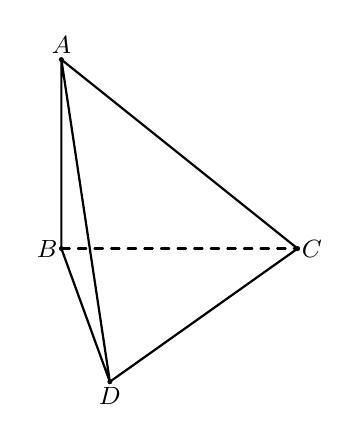
\begin{tikzpicture}[line join = round, line cap = round, thick, font = \small, scale = .6]
	\path
	(0:0) coordinate (B)
	+(0:5) coordinate (C)
	+(-70:3) coordinate (D)
	++(90:4) coordinate (A)
	;
	\draw[dashed]
	(B)--(C)
	;
	\draw
	(A)--(B)--(D)--(C)--cycle
	(A)--(D)
	;
	\foreach \x/\g in {B/180,C/0,D/-90,A/90}
	\fill (\x) circle (1.5pt)
	+(\g:3mm) node {$\x$};
	\end{tikzpicture}
	}
	\loigiai{
	}
\end{ex}
%%==========Câu 12
\begin{ex}
	\immini{
	Cho hình lăng trụ tam giác $ABC.A'B'C'$.Gọi $M$, $N$ lần lượt là trung điểm của $AB$, $AC$. Trong 4 vectơ $\vec{AB}$, $\vec{CB}$, $\vec{B'C'}$, $\vec{A'C'}$ vectơ nào cùng hướng với vectơ $\vec{MN}$
	\choice
	{$\vec{AB}$}
	{$\vec{CB}$}
	{\True $\vec{B'C'}$}
	{$\vec{A'C'}$}
	}{\begin{tikzpicture}[line join = round, line cap = round, thick, font = \small, scale = .7]
	\path
	(0:0) coordinate (A)
	+(0:4) coordinate (C)
	+(-50:2) coordinate (B)
	+(75:3.5) coordinate (A')
	($(A')+(B)-(A)$) coordinate (B')
	($(A')+(C)-(A)$) coordinate (C')
	($(A)!.5!(B)$) coordinate (M)
	($(A)!.5!(C)$) coordinate (N)
	;
	\draw[dashed]
	(A)--(C) (M)--(N)
	;
	\draw
	(A)--(B)--(C)--(C')--(A')--cycle
	(B')--(A') (B')--(B) (B')--(C')
	;
	\foreach \x/\g in {A/180,B/-90,C/0,A'/-180,B'/70,C'/0,M/-135,N/-45}
	\fill (\x) circle (1.5pt)
	+(\g:3mm) node {$\x$};
	\end{tikzpicture}
	}
	\loigiai{
	Vì $MN$ là đường trung bình của tam giác $ABC$ nên $MN$ song song với $BC$. Mà tứ giác $BCC'B'$ là hình bình hành. Do đó $MN$ song song với $B'C'$. Vậy hai vectơ $\vec{MN}$ và $\vec{B'C'}$ cùng hướng.
	}
\end{ex}
%%==========Câu 13
\begin{ex}
	\immini{
	Cho hình hộp $ABCD.A'B'C'D'$.Số các vectơ có điểm đầu, điểm cuối là các đỉnh của hình hộp và bằng vectơ $\vec{AB}$ là
	\choice
	{$1$}
	{$2$}
	{\True $3$}
	{$4$}
	}{\begin{tikzpicture}[line join = round, line cap = round, thick, font = \small, scale = .7]
	\path
	(0:0) coordinate (D')
	+(75:3.5) coordinate (D)
	+(0:3) coordinate (C')
	+(40:2) coordinate (A')
	($(C')+(D)-(D')$) coordinate (C)
	($(D)+(A')-(D')$) coordinate (A)
	($(C')+(A')-(D')$) coordinate (B')
	($(C)+(A)-(D)$) coordinate (B)
	;
	\draw[dashed]
	(A')--(A) (A')--(B') (A')--(D')
	;
	\draw
	(A)--(B)--(B')--(C')--(D')--(D)--cycle
	(C)--(B) (C)--(D) (C)--(C')
	;
	\foreach \x/\g in {D'/-90,C'/-90,D/180,A'/135,C/-45,A/90,B'/0,B/90}
	\fill (\x) circle (1.5pt)
	+(\g:3mm) node {$\x$};
	\end{tikzpicture}
	}
	\loigiai{
	$\vec{AB}=\vec{DC}=\vec{D'C'}=\vec{A'B'}$
	}
\end{ex}
%%==========Câu 14
\begin{ex}
	Cho hình hộp $ABCD.A'B'C'D'$. Trong các khẳng định dưới đây, đâu là khẳng định đúng?
	\choice
	{$\vec{AB}+\vec{AC}+\vec{AD}=\vec{AC'}$}
	{\True $\vec{AB}+\vec{AA'}+\vec{AD}=\vec{AC'}$}
	{$\vec{AB}+\vec{AA'}+\vec{AD}=\vec{AC}$}
	{$\vec{AB}+\vec{AA'}+\vec{AD}=\vec{0}$}
	\loigiai{
	Xét hình hộp $ABCD.A'B'C'D'$ ta có $\vec{AB}+\vec{AA'}+\vec{AD}=\vec{AC'}$
	}
\end{ex}
%%==========Câu 15
\begin{ex}
	Trong không gian cho tam giác $ABC$ có $G$ là trọng tâm và điểm $M$ nằm ngoài mặt phẳng $(ABC)$. Khẳng định nào sau đây là đúng?
	\choice
	{$\vec{MA}+\vec{MB}+\vec{MC}=\vec{0}$}
	{$\vec{GA}+\vec{GB}+\vec{GC}=0$}
	{$\vec{MA}+\vec{MB}+\vec{MC}=\vec{MG}$}
	{\True $\vec{MA}+\vec{MB}+\vec{MC}=3\vec{MG}$}
	\loigiai{
	Vì $G$ là trọng tâm tam giác $ABC$ nên $\vec{MA}+\vec{MB}+\vec{MC}=3\vec{MG}$
	}
\end{ex}
%%==========Câu 16
\begin{ex}
	Cho hình chóp đều $S.ABCD$ tất cả các cạnh bằng $2\sqrt{3}$. Tính độ dài vectơ $\vec{u}=\vec{SA}-\vec{SC}$.
	\choice
	{$\sqrt{3}$}
	{$\sqrt{2}$}
	{\True $2\sqrt{6}$}
	{$2\sqrt{2}$}
	\loigiai{
	Ta có: $|\vec{u}| = |\vec{SA}-\vec{SC}| = |\vec{CA}| = AB\sqrt{2} =2\sqrt{6}$.
	}
\end{ex}
%%==========Câu 17
\begin{ex}
	Cho tứ diện $ABCD$. Mệnh đề nào dưới đây là mệnh đề đúng?
	\choice
	{$\vec{BC}-\vec{BA}=\vec{DA}-\vec{DC}$}
	{$\vec{AC}-\vec{AD}=\vec{BD}-\vec{BC}$}
	{\True $\vec{AB}-\vec{AC}=\vec{DB}-\vec{DC}$}
	{$\vec{AB}-\vec{AD}=\vec{CD}-\vec{CB}$}
	\loigiai{
	Ta có: $\heva{& \vec{AB}-\vec{AC}=\vec{CB} \\& \vec{DB}-\vec{DC}=\vec{CB}}\Rightarrow \vec{AB}-\vec{AC}=\vec{DB}-\vec{DC}$.
	}
\end{ex}
%%==========Câu 18
\begin{ex}
	Cho hình lăng trụ $ABC.A'B'C'$, $M$ là trung điểm của $BB'$. Đặt $\vec{CA}=\vec{a}$, $\vec{CB}=\vec{b}$, $\vec{AA'}=\vec{c}$. Khẳng định nào sau đây đúng?
	\choice
	{$\vec{AM}=\vec{b}+\vec{c}-\dfrac{1}{2}\vec{a}$}
	{$\vec{AM}=\vec{a}-\vec{c}+\dfrac{1}{2}\vec{b}$}
	{$\vec{AM}=\vec{a}+\vec{c}-\dfrac{1}{2}\vec{b}$}
	{\True $\vec{AM}=\vec{b}-\vec{a}+\dfrac{1}{2}\vec{c}$}
	\loigiai{
	\immini{
	Ta có: $\vec{AM}=\vec{AB}+\vec{BM}=\vec{CB}-\vec{CA}+\dfrac{1}{2}\vec{BB'}=\vec{CB}-\vec{CA}+\dfrac{1}{2}\vec{AA'}=\vec{b}-\vec{a}+\dfrac{1}{2}\vec{c}$
	}{\begin{tikzpicture}[line join = round, line cap = round, thick, font = \small, scale = .6]
	\path
	(0:0) coordinate (A)
	+(0:4) coordinate (C)
	+(-50:2) coordinate (B)
	+(75:4) coordinate (A')
	($(A')+(B)-(A)$) coordinate (B')
	($(A')+(C)-(A)$) coordinate (C')
	($(B)!.5!(B')$) coordinate (M)
	;
	\draw[dashed]
	(A)--(C)
	;
	\draw
	(A)--(B)--(C)--(C')--(A')--cycle
	(B')--(A') (B')--(B) (B')--(C') (A)--(M)
	;
	\foreach \x/\g in {A/180,B/-90,C/0,A'/-180,B'/70,C'/0,M/135}
	\fill (\x) circle (1.5pt)
	+(\g:3mm) node {$\x$};
	\end{tikzpicture}
	}
	}
\end{ex}
%%==========Câu 19
\begin{ex}
	Cho hình lập phương $ABCD.A'B'C'D'$ cạnh $a$. Tính độ dài véctơ $\vec{x}=\vec{A'C'}-\vec{A'A}$ theo $a$?
	\choice
	{$a\sqrt{2}$}
	{$\dfrac{a\sqrt{3}}{2}$}
	{$a\sqrt{6}$}
	{\True $a\sqrt{3}$}
	\loigiai{
	Ta có $\vec{x}=\vec{A'C'}-\vec{A'A}=\vec{AC'}=a\sqrt{3}$.
	}
\end{ex}
%%==========Câu 20
\begin{ex}
	\immini{Cho tứ diện $S.ABC$ có $M$, $N$, $P$ là trung điểm của $SA$, $SB$, $SC$. Tìm khẳng định đúng?}
	{\begin{tikzpicture}[line join = round, line cap = round, thick, font = \small, scale = .7]
	\path
	(0:0) coordinate (A)
	+(0:5) coordinate (C)
	+(-70:2) coordinate (B)
	+(65:4) coordinate (S)
	($(S)!.5!(A)$) coordinate (M)
	($(S)!.5!(B)$) coordinate (N)
	($(S)!.5!(C)$) coordinate (P)
	;
	\draw[dashed]
	(A)--(C) (M)--(P)
	;
	\draw
	(A)--(B)--(C)--(S)--cycle
	(S)--(B) (M)--(N)--(P)
	;
	\foreach \x/\g in {A/180,C/0,B/-90,S/45,M/135,N/-45,P/45}
	\fill (\x) circle (1.5pt)
	+(\g:3mm) node {$\x$};
	\end{tikzpicture}}
	\choice
	{$\vec{AB}=\dfrac{1}{2}\left(\vec{PN}-\vec{PM}\right)$}
	{$\vec{AB}=\vec{PN}-\vec{PM}$}
	{$\vec{AB}=2\left(\vec{PM}-\vec{PN}\right)$}
	{\True $\vec{AB}=2\left(\vec{PN}-\vec{PM}\right)$}
	\loigiai{
	Ta có: $\vec{AB}=2\vec{MN}=2\left(\vec{PN}-\vec{PM}\right)$.
	}
\end{ex}
%%==========Câu 21
\begin{ex}
	\immini{Cho tứ diện $S.ABC$ có đáy là tam giác đều cạnh $a$, $SB$ vuông góc với đáy và $SB=\sqrt{3}a$. Góc giữa hai vectơ $(\vec{AB},\vec{AS})$ là}
	{\begin{tikzpicture}[line join = round, line cap = round, thick, font = \small, scale = .7]
	\path
	(0:0) coordinate (B)
	+(0:5) coordinate (C)
	+(-50:3) coordinate (A)
	+(90:4) coordinate (S)
	;
	\draw[dashed]
	(B)--(C)
	;
	\draw
	(S)--(B)--(A)--(C)--cycle
	(S)--(A)
	\foreach \x/\y/\z in {S/B/C,S/B/A}{
	pic[draw, angle radius = 8pt]{right angle = \x--\y--\z}
	}
	;
	\foreach \x/\g in {B/180,C/0,A/-90,S/90}
	\fill (\x) circle (1.5pt)
	+(\g:3mm) node {$\x$};
	\end{tikzpicture}}
	\choice
	{\True $60^\circ$}
	{$30^\circ$}
	{$45^\circ$}
	{$90^\circ$}
	\loigiai{
	Ta có: $\left(\vec{AB},\vec{AS}\right)=\widehat{SAB}$.\\
	Xét $\triangle SBA$ vuông tại $B$ ta có: $\tan \left(\widehat{SAB}\right)=\dfrac{SB}{AB}=\sqrt{3}$. Suy ra: $\left(\vec{AB},\vec{AS}\right)=60^\circ$
	}
\end{ex}
%%==========Câu 22
\begin{ex}
	Cho hình chóp $S.ABC$ có $AB=4$, $\widehat{BAC}=60^\circ$, $\vec{AB} \cdot \vec{AC}=6$. Khi đó độ dài $\vec{AC}$ là
	\choice
	{\True $3$}
	{$6$}
	{$4$}
	{$12$}
	\loigiai{
	Ta có: $\vec{AB} \cdot \vec{AC}=AB \cdot AC \cdot \cos \widehat{BAC}\Leftrightarrow 6=4 \cdot AC \cdot \cos 60^\circ \Leftrightarrow AC=3$.
	}
\end{ex}
%%==========Câu 23
\begin{ex}
	Trong không gian cho vectơ $\vec{AB}$. Khi đó:
	\choice
	{Giá của vectơ $\vec{AB}$ là $\vec{AB}$}
	{Giá của vectơ $\vec{AB}$ là $\left| \vec{AB} \right|$}
	{\True Giá của vectơ $\vec{AB}$ là đường thẳng $AB$}
	{Giá của vectơ $\vec{AB}$ là đoạn thẳng $AB$}
	\loigiai{
	Giá của vectơ $\vec{AB}$ là đường thẳng $AB$.
	}
\end{ex}
%%==========Câu 24
\begin{ex}
	Cho hình hộp chữ nhật $ABCD.A'B'C'D'$. Trong các vectơ dưới đây, vectơ nào cùng phương với vectơ $\vec{AB}$?
	\choice
	{Vectơ$\vec{AD}$}
	{Vectơ$\vec{CC'}$}
	{Vectơ$\vec{BD}$}
	{\True Vectơ$\vec{CD}$}
	\loigiai{
	$AB \parallel CD$ nên $\vec{AB}$ và $\vec{CD}$ cùng phương.
	}
\end{ex}
%%==========Câu 25
\begin{ex}
	Cho hình hộp $ABCD.A'B'C'D'$. Vectơ $\vec{u}=\vec{A'A}+\vec{A'B'}+\vec{A'D'}$ bằng vectơ nào dưới đây?
	\choice
	{\True $\vec{A'C}$}
	{$\vec{CA'}$}
	{$\vec{AC'}$}
	{$\vec{C'A}$}
	\loigiai{
	Do $A'B'BA$ là hình bình hành nên $\vec{A'A}+\vec{A'B'}=\vec{A'B}$. Lại có, $A'BCD'$ cũng là hình bình hành nên $\vec{A'B}+\vec{A'D'}=\vec{A'C}$. Vậy $\vec{A'A}+\vec{A'B'}+\vec{A'D'}=\vec{A'C}$
	}
\end{ex}
%%==========Câu 26
\begin{ex}
	Cho hình lăng trụ tam giác $ABC.A'B'C'$. Đặt $\vec{AA'}=\vec{a}$, $\vec{AB}=\vec{b}$, $\vec{AC}=\vec{c}$, $\vec{BC}=\vec{d}$. Trong các biểu thức vec tơ sau đây, biểu thức nào là đúng?
	\choice
	{$\vec{a}=\vec{b}+\vec{c}$}
	{$\vec{a}+\vec{b}+\vec{c}+\vec{d}=\vec{0}$}
	{\True $\vec{b}-\vec{c}+\vec{d}=\vec{0}$}
	{$\vec{a}+\vec{b}+\vec{c}=\vec{d}$}
	\loigiai{
	Ta có: $\vec{b}-\vec{c}+\vec{d}=\vec{AB}-\vec{AC}+\vec{BC}=\vec{CB}+\vec{BC}=\vec{0}$.
	}
\end{ex}
%%==========Câu 27
\begin{ex}
	Cho lập phương $ABCD.A'B'C'D'$ có độ dài mỗi cạnh bằng $1$. Tính độ dài của vectơ $\vec{AC}+\vec{C'D'}$.
	\choice
	{$\sqrt{3}$}
	{$\sqrt{2}$}
	{\True $1$}
	{$2\sqrt{2}$}
	\loigiai{
	Ta có: $A'C'CA$ là hình chữ nhật nên $\vec{A'C'}=\vec{AC}$.\\
	Khi đó, $\vec{AC}+\vec{C'D'}=\vec{A'C'}+\vec{C'D'}=\vec{A'D'}$. Vậy $\left| \vec{AC}+\vec{C'D'} \right| =\left| \vec{A'D'} \right| =A'D'=1$
	}
\end{ex}
%%==========Câu 28
\begin{ex}
	Cho $O$ là tâm hình bình hành $ABCD$. Hỏi vectơ $\left(\vec{AO}-\vec{DO}\right)$ bằng vectơ nào?
	\choice
	{$\vec{BA}$}
	{\True $\vec{AD}$}
	{$\vec{DC}$}
	{$\vec{AC}$}
	\loigiai{
	Ta có: $\vec{AO}-\vec{DO}=\vec{AO}+\vec{OD}=\vec{AD}$.
	}
\end{ex}
%%==========Câu 29
\begin{ex}
	Cho ba điểm phân biệt $A$, $B$, $C$. Nếu $\vec{AB}=-3\vec{AC}$ thì đẳng thức nào dưới đây đúng?
	\choice
	{$\vec{BC}=-4\vec{AC}$}
	{$\vec{BC}=-2\vec{AC}$}
	{$\vec{BC}=2\vec{AC}$}
	{\True $\vec{BC}=4\vec{AC}$}
	\loigiai{
	Ta có: $\vec{AB}=-3\vec{AC}\Leftrightarrow \vec{CB}-\vec{CA}=-3\vec{AC}\Leftrightarrow \vec{AC}+3\vec{AC}=-\vec{CB}\Leftrightarrow \vec{BC}=4\vec{AC}$.
	}
\end{ex}
%%==========Câu 30
\begin{ex}
	Cho tam giác $ABC$ có điểm $O$ thỏa mãn: $\left| \vec{OA}+\vec{OB}-2\vec{OC} \right| = \left| \vec{OA}-\vec{OB} \right|$. Khẳng định nào sau đây là đúng?
	\choice
	{Tam giác $ABC$ đều}
	{Tam giác $ABC$ cân tại $C$}
	{\True Tam giác $ABC$ vuông tại $C$}
	{Tam giác $ABC$ cân tại $B$}
	\loigiai{
	Gọi $M$ là trung điểm $AB$, ta có $\vec{OA}+\vec{OB}=2\vec{OM}$.\\
	Do đó, $\left| \vec{OA}+\vec{OB}-2\vec{OC} \right| =\left| \vec{OA}-\vec{OB} \right|\Leftrightarrow \left| 2\vec{OM}-2\vec{OC} \right| =\left| \vec{BA} \right|\Leftrightarrow 2\left| \vec{CM} \right| =BA\Leftrightarrow CM=\dfrac{1}{2}BA$ \hfill $(1)$\\
	Vì $M$ là trung điểm $AB$ nên $CM$ là đường trung tuyến của $\triangle ABC$, Từ $(1)$ suy ra, tam giác $\triangle ABC$ vuông tại $C$.
	}
\end{ex}
%%==========Câu 31
\begin{ex}
	Cho hình hộp $ABCD.A'B'C'D'$. Đẳng thức nào dưới đây là đúng?
	\choice
	{$\vec{AC'}=\vec{AB}+\vec{AD}+\vec{AC}$}
	{$\vec{AC'}=\vec{AA'}+\vec{AD}+\vec{AC}$}
	{\True $\vec{AC'}=\vec{AB'}+\vec{AD}$}
	{$\vec{AC'}=\vec{AC}+\vec{AB}+\vec{AA'}$}
	\loigiai{
	Do $AB'C'D$ là hình bình hành nên $\vec{AC'}=\vec{A'B'}+\vec{AD}$.
	}
\end{ex}
%%==========Câu 32
\begin{ex}
	Cho hình lập phương $ABCD.A'B'C'D'$ có độ dài cạnh bằng $a$. Tính độ dài của vectơ $\vec{AD'}+\vec{BA'}$.
	\choice
	{$\sqrt{3}a$}
	{$\sqrt{2}a$}
	{\True $\sqrt{6}a$}
	{$2\sqrt{3}a$}
	\loigiai{
	Gọi $O'$ là tâm của hình vuông $A'B'C'D'$.\\
	Ta có $ABC'D'$ là hình bình hành nên $\vec{AD'}=\vec{BC'}$, do đó $\vec{BA'}+\vec{AD'}=\vec{BA'}+\vec{BC'}=2\vec{BO'}$.\\
	Tam giác $BA'C'$ là tam giác đều cạnh $a\sqrt{2}$ nên $BO'=\dfrac{\sqrt{3}}{2}a\sqrt{2}=\dfrac{\sqrt{6}}{2}a$.\\
	Từ đó độ dài của vectơ $\vec{AD'}+\vec{BA'}$ bằng $\sqrt{6}a$.
	}
\end{ex}
%%==========Câu 33
\begin{ex}%[2H2H1-4]
	\immini{
	Trong điện trường đều, lực tĩnh điện $\vec{F}$ (đơn vị: N) tác dụng lên điện tích điểm có điện tích $q$ (đơn vị: C) được tính theo công thức $\vec{F}=q \cdot \vec{E}$, trong đó $\vec{E}$ là cường độ điện trường (đơn vị: N/C). Tính độ lớn của lực tĩnh điện tác dụng lên điện tích điểm khi $q=10^{-9}$ C và độ lớn điện trường $E=10^5$ N/C.
	\choice
	{$10^{-3}$ N}
	{$10^{4}$ N}
	{$10^{-14}$ N}
	{\True $10^{-4}$ N}
	}{\hspace{1cm}
	\begin{tikzpicture}[scale=.7]
	\def\drong{3} % khoảng cách giữa 2 thanh
	\def\drog{0.3} % một nữa độ rộng của thanh
	\def\num{8}
	\filldraw [green!5, draw=green!80!black] ($(0,0)+(-\drog,\drog)$) rectangle ($(0,0)+(\num,0)+(\drog,-\drog)$)
	($(0,-\drong)+(-\drog,\drog)$) rectangle ($(0,-\drong)+(\num,0)+(\drog,-\drog)$);
	\foreach \a in {0,1,...,\num}{
	\draw[->,>=Latex] ($(0,0)+(\a,0)$)node[red]{$+$} ($(0,0)+(\a,0)+(0,-\drog)$)-- ($(0,-0.5*\drong)+(\a,0)$);
	\draw ($(0,-0.5*\drong)+(\a,0)$) -- ($(0,-\drong)+(\a,0)+(0,\drog)$) ($(0,-\drong)+(\a,0)$)node[red]{$-$} ;}
	\draw[->,>=Latex] (3.5,-0.4*\drong)--++(-90:1)node[below]{$\vec{F}$};
	\filldraw [green!5, draw=green!80!black] (3.5,-0.4*\drong)node[green!90!black]{$+$} circle (0.2cm) ;
	\draw (4.5,-0.5*\drong)node{$M$} (8.5,-0.5*\drong)node[red]{$\vec{E}$};
	\end{tikzpicture}
	}
	\loigiai{
	Từ công thức $\vec{F}=q \cdot \vec{E}$ suy ra $\begin{aligned}[t]
	|\vec{F}| & =q|\vec{E}| \\
	 & =10^{-9} \cdot 10^5 \\
	 & =10^{-4} \text{N}.
	\end{aligned}$\\
	Vậy độ lớn của lực tĩnh điện tác dụng lên điện tích điểm là $10^{-4}$ N.
	}
\end{ex} \dongcham{4}
\Closesolutionfile{ans}
\textbf{PHẦN II.} \textit{Câu trắc nghiệm đúng sai. Trong mỗi ý a), b), c), d) ở mỗi câu, học sinh chọn đúng hoặc sai.}\\
\Opensolutionfile{ans}[ans/2H2-B1-d1-2]
%%==========Câu 34
\begin{ex}
	\immini{Cho hình hộp chữ nhật $ABCD.A'B'C'D'$ có cạnh $AB=a$; $AD=a\sqrt{3}$; $AA'=2a$. Xét tính đúng, sai của các khẳng định sau:
	\choiceTF
	{$\vec{AB'}+\vec{CD'}=\vec{0}$}
	{\True $\vec{A'D}+\vec{CB'}=\vec{0}$}
	{$\big|\vec{AB}+\vec{AD}\big|=a\sqrt{5}$}
	{\True $\big|\vec{AB}+\vec{A'D'}+\vec{CC'}\big|=2\sqrt{2}a$}}{
	\begin{tikzpicture}[scale=0.6, font=\footnotesize, line join=round, line cap=round]
	\def\h{4}
	\foreach \x\y\t in {0/0/A,-1/-1.1/B,4.6/-1.1/C}
	\coordinate (\t) at (\x,\y);
	\coordinate (D) at ($(A)+(C)-(B)$);
	\coordinate (A') at ($(A)+(0,3.2)$);
	\coordinate (B') at ($(B)+(0,3.2)$);
	\coordinate (C') at ($(C)+(0,3.2)$);
	\coordinate (D') at ($(D)+(0,3.2)$);
	\draw (B')--(A')--(D')--(C')--(B')--(B)--(C)--(D)--(D') (C')--(C);
	\draw[dashed](B)--(A)--(D) (A)--(A');
	\foreach \t/\g in {A/170,B/-150,C/-70,D/0,A'/100,B'/170,C'/-20,D'/50}
	\draw[fill=black] (\t) circle(1pt)
	node[shift={(\g:7pt)}]{$\t$};
	\end{tikzpicture}}
	\loigiai{\begin{enumerate}[a)]
	\item $\vec{AB'}$ và $\vec{CD'}$ không đối nhau nên $\vec{AB'}+\vec{CD'} \ne \vec{0}$
	\item $\vec{A'D}$ và $\vec{CB'}$ đối nhau nên $\vec{AB'}+\vec{CD'} = \vec{0}$
	\item $\big|\vec{AB}+\vec{AD}\big|=\big|\vec{AC}\big|=AC=\sqrt{AB^2+AD^2}=2a$
	\item $\big|\vec{AB}+\vec{A'D'}+\vec{CC'}\big|=\big|\vec{AB}+\vec{AD}+\vec{AA'}\big|=AC'=\sqrt{AB^2+AD^2+AA^2}=2\sqrt{2}a$
	\end{enumerate}}
\end{ex} \dongcham{8}
%%==========Câu 35
\begin{ex}%[2H2H1-2]
	\immini{Cho hình lập phương $ABCD.A'B'C'D'$ có cạnh bằng $a$. Xét tính đúng, sai của các khẳng định sau:
	\choiceTF
	{\True $\vec{B'B} - \vec{DB} = \vec{B'D}$}
	{$\vec{BA}+\vec{BC}+\vec{BB'}=\vec{BD}$}
	{$\big|\vec{BA}+\vec{BC}+\vec{BB'}\big|=a\sqrt{2}$}
	{\True $\big|\vec{BC}-\vec{BA}+\vec{C'A}\big|=a$}
	}{
	\begin{tikzpicture}[scale=0.6, font=\footnotesize, line join=round, line cap=round]
	\def\h{4}
	\foreach \x\y\t in {0/0/A,-1/-1.1/B,2.6/-1.1/C}
	\coordinate (\t) at (\x,\y);
	\coordinate (D) at ($(A)+(C)-(B)$);
	\coordinate (A') at ($(A)+(0,3.2)$);
	\coordinate (B') at ($(B)+(0,3.2)$);
	\coordinate (C') at ($(C)+(0,3.2)$);
	\coordinate (D') at ($(D)+(0,3.2)$);
	\draw (B')--(A')--(D')--(C')--(B')--(B)--(C)--(D)--(D') (C')--(C);
	\draw[dashed](B)--(A)--(D) (A)--(A');
	\foreach \t/\g in {A/170,B/-150,C/-70,D/0,A'/100,B'/170,C'/-20,D'/50}
	\draw[fill=black] (\t) circle(1pt)
	node[shift={(\g:7pt)}]{$\t$};
	\end{tikzpicture}}
	\loigiai{
	\immini{\vspace*{-3mm}
	\begin{listEX}
	\item Ta có \begin{eqnarray*}
	\vec{B'B} - \vec{DB} &=& \vec{B'B} + \left( - \vec{DB} \right) \\
	&=& \vec{B'B} + \vec{BD} \\
	&=& \vec{B'D}.
	\end{eqnarray*}
	\item Áp dụng quy tắc hình hộp ta có $\vec{BA}+\vec{BC}+\vec{BB'}=\vec{BD'}$.\\
	\item $\big|\vec{BA}+\vec{BC}+\vec{BB'}\big|=\big|\vec{BD'}\big|=BD'=a\sqrt{3}$
	\item Ta có $\vec{BC}-\vec{BA}+\vec{C'A}=\vec{AC}+\vec{C'A}=\vec{C'C}$.\\
	Do đó $\big|\vec{BC}-\vec{BA}+\vec{C'A}\big|=C'C=a$
	\end{listEX}}
	{
	\begin{tikzpicture}[scale=0.6, font=\footnotesize, line join=round, line cap=round]
	\def\h{4}
	\foreach \x\y\t in {0/0/A,-1/-1.1/B,2.6/-1.1/C}
	\coordinate (\t) at (\x,\y);
	\coordinate (D) at ($(A)+(C)-(B)$);
	\coordinate (A') at ($(A)+(0,3.2)$);
	\coordinate (B') at ($(B)+(0,3.2)$);
	\coordinate (C') at ($(C)+(0,3.2)$);
	\coordinate (D') at ($(D)+(0,3.2)$);
	\draw (B')--(A')--(D')--(C')--(B')--(B)--(C)--(D)--(D') (C')--(C);
	\draw[dashed](B)--(A)--(D) (A)--(A');
	\foreach \t/\g in {A/170,B/-150,C/-70,D/0,A'/100,B'/170,C'/-20,D'/50}
	\draw[fill=black] (\t) circle(1pt)
	node[shift={(\g:7pt)}]{$\t$};
	\end{tikzpicture}}
	}
\end{ex} \dongcham{14}
%%==========Câu 36
\begin{ex}%[2H2N1-2]
	\immini{Cho hình lăng trụ tam giác $A B C.A' B' C'$ có $\vec{A A'}=\vec{a}$, $\vec{A B}=\vec{b}$ và $\vec{A C}=\vec{c}$. Gọi $M$ là trung điểm của $BC$. Xét tính đúng, sai của các khẳng định sau:
	\choiceTF
	{\True $\vec{B'C}=-\vec{a}-\vec{b}+\vec{c}$}
	{\True $\vec{BC'}=\vec{a}-\vec{b}+\vec{c}$}
	{$\vec{AM}=\vec{b}+\vec{c}$}
	{\True $\vec{A'M}=-\vec{a}+\dfrac{1}{2}\vec{b}+\dfrac{1}{2}\vec{c}$}
	}{
	\begin{tikzpicture}[scale=0.8, font=\footnotesize,>=stealth]
	\path
	(0,0) coordinate (A)
	(4,0) coordinate (C)
	(1.5,-1.5) coordinate (B)
	($(A)+(0.4,3)$)coordinate (A')
	($(B)+(0.4,3)$)coordinate (B')
	($(C)+(0.4,3)$)coordinate (C')
	($(B)!1/2!(C)$)coordinate (M)
	;
	\draw (B)--(C)--(C')--(B')--(B)--(A)--(A')--(B') (A')--(C');
	\draw[dashed] (C)--(A)--(M)--(A');
	\foreach \x/\g in {A/180,B/-45,C/0,A'/180,B'/-30,C'/0,M/-90}\draw[fill=black] (\x) circle (.04) +(\g:.4)node{\footnotesize$\x$};
	\end{tikzpicture}}
	\loigiai{
	\immini{\begin{enumerate}[a)]
	\item $\vec{B'C}=\vec{B'A'}+\vec{A'C'}+\vec{C'C}=-\vec{AB}+\vec{AC}-\vec{AA'}$ hay $\vec{B'C}=-\vec{a}-\vec{b}+\vec{c}$;
	\item $\vec{BC'}=\vec{BB'}+\vec{B'A'}+\vec{A'C'}=\vec{AA'}-\vec{AB}+\vec{AC}$ hay $\vec{BC'}=\vec{a}-\vec{b}+\vec{c}$;
	\item Ta có $\vec{AB}+\vec{AC}=2\vec{AM}$, suy ra $\vec{AM}=\dfrac{1}{2}\vec{AB}+\dfrac{1}{2}\vec{AC}=\dfrac{1}{2}\vec{b}+\dfrac{1}{2}\vec{c}$
	\item $\vec{A'M}=\vec{A'A}+\vec{AM}=\vec{A'A}+\dfrac{1}{2}\vec{AB}+\dfrac{1}{2}\vec{AC}=-\vec{a}+\dfrac{1}{2}\vec{b}+\dfrac{1}{2}\vec{c}$
	\end{enumerate}}{\begin{tikzpicture}[scale=0.6, font=\footnotesize,>=stealth]
	\path
	(0,0) coordinate (A)
	(4,0) coordinate (C)
	(1.5,-1.5) coordinate (B)
	($(A)+(0.4,3)$)coordinate (A')
	($(B)+(0.4,3)$)coordinate (B')
	($(C)+(0.4,3)$)coordinate (C')
	($(B)!1/2!(C)$)coordinate (M)
	;
	\draw (B)--(C)--(C')--(B')--(B)--(A)--(A')--(B') (A')--(C');
	\draw[dashed] (C)--(A)--(M)--(A');
	\foreach \x/\g in {A/180,B/-45,C/0,A'/180,B'/-30,C'/0,M/-90}\draw[fill=black] (\x) circle (.04) +(\g:.4)node{\footnotesize$\x$};
	\end{tikzpicture}}
	}
\end{ex} \dongcham{14}
%%==========Câu 37
\begin{ex}
	\immini{
	Cho tứ diện $ABCD$. Gọi $M$, $N$ lần lượt là trung điểm của các cạnh $AD$ và $BC$, $I$ là trung điểm $MN$. Xét tính đúng, sai của các khẳng định sau:
	\choiceTF
	{$\vv{A B}-\vv{C D}=\vv{A C}-\vv{B D}$}
	{\True $\vec{AB} + \vec{CD} = \vec{AD} + \vec{CB}$}
	{\True $\vec{AB} + \vec{DC}=2\vec{MN}$}
	{\True $\vec{IA} + \vec{IB} + \vec{IC} + \vec{ID} = \vec{0}$}
	}{
	\vspace*{-3mm}
	\begin{tikzpicture}[scale=0.5, font=\footnotesize, line join=round, line cap=round]
	\foreach \x\y\t in {0/0/B,6/0/D,1.5/-2/C,1.5/5/A}
	\coordinate (\t) at (\x,\y);
	\coordinate (M) at ($(A)!1/2!(D)$);
	\coordinate (N) at ($(B)!1/2!(C)$);
	\coordinate (I) at ($(M)!1/2!(N)$);
	\draw (A)--(B)--(C)--(D)--(A)--(C);
	\draw[dashed] (D)--(I)--(A) (B)--(I)--(C) (M)--(N) (B)--(D);
	\foreach \t/\g in {A/90,B/180,C/-90,D/0,M/0,N/180,I/20} \draw (\t) node[shift={(\g:10pt)}]{$\t$};
	\end{tikzpicture}}
	\loigiai{
	\begin{enumerate}
	\item Sử dụng quy tắc ba điểm và quy tắc hiệu, ta có
	 \begin{align*}
	 \vv{A B}-\vv{C D} & \ =\left(\vv{A C}+\vv{C B}\right)-\vv{C D} \\
	 & \ =\vv{A C}+\left(\vv{C B}-\vv{C D}\right) \\
	 & \ =\vv{A C}+\vv{D B} \\
	 & \ =\vv{A C}-\vv{B D}.
	 \end{align*}
	\item Theo quy tắc ba điểm, ta có $\vec{AB} = \vec{AD} + \vec{DB}$. Do đó
	 \begin{eqnarray*}
	 \vec{AB} + \vec{CD} &=& \vec{AD} + \vec{DB} + \vec{CD} \\
	 &=&\vec{AD}+ \left( \vec{CD} + \vec{DB} \right) \\
	 &=& \vec{AD} + \vec{CB}.
	 \end{eqnarray*}
	\item Ta có
	\item
	\end{enumerate}
	}
\end{ex} \dongcham{8}
%%==========Câu 38
\begin{ex}
	\immini
	{
	Một chiếc ô tô được đặt trên mặt đáy dưới của một khung sắt có dạng hình hộp chữ nhật với đáy trên là hình chữ nhật $ABCD$, mặt phẳng $(ABCD)$ song song với mặt phẳng nằm ngang. Khung sắt đó được buộc vào móc $E$ của chiếc cần cẩu sao cho các đoạn dây cáp $EA$, $EB$, $EC$, $ED$ có độ dài bằng nhau và cùng tạo với mặt phẳng $(ABCD)$ một góc bằng $60^\circ$. Chiếc cần cẩu kéo khung sắt lên theo phương thẳng đứng. Biết rằng các lực căng $\vec{F_1}$, $\vec{F_2}$, $\vec{F_3}$, $\vec{F_4}$ đều có cường độ là $4700$ N và trọng lượng của khung sắt là $3000$ N.
	\choiceTF
	{$\vec{F_1}+\vec{F_2}=\vec{F_3}+\vec{F_4}$}
	{\True $\vec{F_1}+\vec{F_3}=\vec{F_2}+\vec{F_4}$}
	{\True $\big|\vec{F_1}+\vec{F_3}\big|=8141$ N (\textit{làm tròn đến hàng đơn vị})}
	{Trọng lượng của chiếc xe ô tô là $16282$ N (\textit{làm tròn đến hàng đơn vị})}
	}
	{\hspace{1cm}
	\includegraphics[scale=.09]{images/xe-1.jpg}
	}
	\loigiai{
	Lấy các điểm $M$, $N$, $P$, $Q$ lần lượt trên các tia $EA$, $EB$, $EC$, $ED$ sao cho
	\[
	\vec{EM} = \vec{F_1},\ \vec{EN} = \vec{F_2},\ \vec{EP} = \vec{F_3},\ \vec{EQ} = \vec{F_4}.
	\]
	Do các lực căng $\vec{F_1}$, $\vec{F_2}$, $\vec{F_3}$, $\vec{F_4}$ đều có cường độ là $4700$ N nên $EM = EN = EP = EQ = 4700$.
	\begin{center}
	\begin{tikzpicture}[line join=round, line cap = round, >=stealth, scale=.8,font=\footnotesize,transform shape]
	\foreach \x/\y/\z/\g in
	{
	-3/0/A/180, -1/-1/B/-90, 3/0/C/0, 1/1/D/45, 0/4/E/90
	}
	\draw[fill=black] (\x,\y) circle(1pt) coordinate (\z) ($(\z)+(\g:3.5mm)$) node{$\z$};
	\path
	($(E)!.75!(A)$) coordinate (M)
	($(E)!.75!(B)$) coordinate (N)
	($(E)!.75!(C)$) coordinate (P)
	($(E)!.75!(D)$) coordinate (Q)
	($(M)!.5!(P)$) coordinate (O)
	;
	\draw (E)--(A)--(B)--(E)--(C)--(B) (M)--(N)--(P);
	\draw[dashed] (M)--(P)--(Q)--(M) (N)--(Q) (O)--(E)--(D)--(C) (A)--(D);
	\foreach \x/\g in {M/135, N/-45,P/45,Q/45,O/135}
	\draw[fill = white] (\x) circle(1pt) ($(\x)+(\g:3mm)$) node{$\x$};
	\end{tikzpicture}
	\end{center}
	\begin{enumerate}[a)]
	\item Ta có
	 \begin{itemize}
	 \item [$\bullet$] $\vec{F_1}+\vec{F_2}=\vec{EM}+\vec{EN}=2\vec{EH}$, với $H$ là trung điểm của $MN$.
	 \item [$\bullet$] $\vec{F_3}+\vec{F_4}=\vec{EP}+\vec{EQ}=2\vec{EK}$, với $K$ là trung điểm của $PQ$.
	 \end{itemize}
	 Suy ra $\vec{F_1}+\vec{F_2}\ne \vec{F_3}+\vec{F_4}$
	\item Ta có
	 \begin{itemize}
	 \item [$\bullet$] $\vec{F_1}+\vec{F_3}=\vec{EM}+\vec{EP}=2\vec{EO}$, với $O$ là trung điểm của $MP$.
	 \item [$\bullet$] $\vec{F_2}+\vec{F_4}=\vec{EN}+\vec{EQ}=2\vec{EO}$, với $O$ là trung điểm của $MP$.
	 \end{itemize}
	 Suy ra $\vec{F_1}+\vec{F_3}=\vec{F_2}+\vec{F_4}$.
	\item $\big|\vec{F_1}+\vec{F_3}\big|=\big|2\vec{EO}\big|=2EO$.\\
	 Theo giả thiết, góc giữa $EA$ với $(ABCD)$ bằng $60^\circ$, suy ra góc giữa $EM$ với $(MNPQ)$ cũng bằng $60^\circ$ hay $\widehat{SMO}=60^\circ$.\\
	 Xét $\triangle EMO$ có $EM=4700$, $\widehat{SMO}=60^\circ$. Suy ra $EO = EM \sin 60^\circ = 2350\sqrt{3}$.\\
	 Từ đây, ta tính được $\big|\vec{F_1}+\vec{F_3}\big|=2EO=8141$ N.
	\item Gọi $\vec{P}$ là trọng lực tác dụng lên cả hệ, do $O$ là trung điểm $MP$, $NQ$ nên ta có:
	 \begin{eqnarray*}
	 & \vec{P} & = \vec{F_1}+\vec{F_2}+\vec{F_3}+\vec{F_4}\\
	 & & = \vec{EM} + \vec{EN} + \vec{EP} + \vec{EQ}\\
	 & & = \vec{EO} + \vec{OM} + \vec{EO} + \vec{ON} + \vec{EO} + \vec{OP} + \vec{EO} + \vec{OQ}\\
	 & & = 4\vec{EO} + \left(\vec{OM} + \vec{OP}\right) + \left(\vec{ON} + \vec{OQ}\right)\\
	 & & = 4\vec{EO}.
	 \end{eqnarray*}
	 Suy ra trọng lượng của toàn bộ hệ là $\left| \vec{P} \right| = 4\left| \vec{EO}\right| = 4EO = 9400\sqrt{3}$ N.\\
	 Do trọng trượng khung sắt là $3000$ N nên trọng lượng của xe ô tô là $9400\sqrt{3} - 3000 \approx 13281$ N.
	\end{enumerate}
	}
\end{ex} \dongcham{14}
%%==========Câu 39
\begin{ex}
	\immini{Cho tứ diện $ABCD$ có $AB=AC=AD=a$ và $\widehat{BAC}=\widehat{BAD}=60^\circ ,\widehat{CAD}=90^\circ $. Gọi $I$ là điểm trên cạnh $AB$ sao cho $AI=3IB$ và $J$ là trung điểm của $CD$. Gọi $\alpha $ là góc giữa hai vectơ $\vec{AB}$ và $\vec{IJ}$.
	\choiceTF
	{\True Tam giác $BCD$ vuông cân}
	{$\vec{IJ}=\dfrac{1}{2}\vec{AC}+\dfrac{1}{2}\vec{AD}+\dfrac{3}{2}\vec{AB}$}
	{$\vec{AB} \cdot \vec{AC}+\vec{AC} \cdot \vec{AD}+\vec{AD} \cdot \vec{AB}=\dfrac{a^2}{2}$}
	{\True $\cos \alpha =-\dfrac{\sqrt{5}}{5}$}
	}{\begin{tikzpicture}[line join = round, line cap = round, thick, font = \small, scale = .7]
	\path
	(0:0) coordinate (B)
	+(0:5) coordinate (C)
	+(-70:2) coordinate (D)
	+(75:4) coordinate (A)
	($(B)!1/4!(A)$) coordinate (I)
	($(C)!.5!(D)$) coordinate (J)
	;
	\draw[dashed]
	(B)--(C) (I)--(J)
	;
	\draw
	(A)--(B)--(D)--(C)--cycle
	(A)--(D)
	;
	\foreach \x/\g in {B/180,C/0,D/-90,A/90,I/135,J/-45}
	\fill (\x) circle (1.5pt)
	+(\g:3mm) node {$\x$};
	\end{tikzpicture}}
	\loigiai{
	\begin{enumerate}[a)]
	\item Tam giác $ABC$, $ABD$ đều cạnh bằng $a$, tam giác $ACD$ vuông cân đỉnh $A\Rightarrow CD=a\sqrt{2}$. Vậy tam giác $BCD$ có $BC=BD=a,CD=a\sqrt{2}$ nên tam giác $BCD$ vuông cân.
	\item $\vec{IJ}=\vec{IA}+\vec{AJ}=-\dfrac{3}{4}\vec{AB}+\dfrac{1}{2}\left(\vec{AC}+\vec{AD}\right)=\dfrac{1}{2}\vec{AC}+\dfrac{1}{2}\vec{AD}-\dfrac{3}{4>}\vec{AB}$.
	\item Ta có: $\vec{AC} \cdot \vec{AD}=0$, $\vec{AB} \cdot \vec{AD}=AB \cdot AD \cdot \cos 60^\circ =\dfrac{a^2}{2}$, $\vec{AC} \cdot \vec{AB}=\dfrac{a^2}{2}$. Suy ra $\vec{AB} \cdot \vec{AC}+\vec{AC} \cdot \vec{AD}+\vec{AD} \cdot \vec{AB}=a^2$.\\
	\item $IJ^2=\vec{IJ}^2=\dfrac{1}{4}{{\left(\vec{AC}+\vec{AD}-\dfrac{3}{2}\vec{AB}\right)}^2}
	 =\dfrac{1}{4}\left(\dfrac{17}{4}a^2+2\vec{AC} \cdot \vec{AD}-3\vec{AC} \cdot \vec{AB}-3\vec{AB} \cdot \vec{AD}\right)
	 =\dfrac{5a^2}{16}\Rightarrow IJ=\dfrac{a\sqrt{5}}{4}$.\\
	 $\vec{IJ} \cdot \vec{AB}=\dfrac{1}{2}\left(\vec{AC}+\vec{AD}-\dfrac{3}{2}\vec{AB}\right) \cdot \vec{AB}= \dfrac{1}{2}\left(\vec{AC} \cdot \vec{AB}+\vec{AD} \cdot \vec{AB}-\dfrac{3}{2}{{\vec{AB}}^2}\right)=-\dfrac{a^2}{4}$.\\
	 $\cos \left(\vec{IJ},\vec{AB}\right)=\dfrac{\vec{IJ} \cdot \vec{AB}}{IJ \cdot AB}=\dfrac{-\dfrac{a^2}{4}}{\dfrac{a\sqrt{5}}{4} \cdot a}=-\dfrac{\sqrt{5}}{5}$.
	\end{enumerate}
	}
\end{ex}
%%==========Câu 40
\begin{ex}
	\immini{Cho tứ diện $ABCD$. Gọi $M$, $N$, $P$, $Q$, $R$, $S$, $G$ lần lượt là trung điểm các đoạn thẳng $AB$, $CD$, $AC$, $BD$, $AD$, $BC$, $MN$.
	\choiceTF
	{\True $\vec{MR}=\vec{SN}$}
	{\True $\vec{GA}+\vec{GB}+\vec{GC}+\vec{GD}=\vec{0}$}
	{$2\vec{PQ}=\vec{AB}+\vec{AC}+\vec{AD}$}
	{\True $|\vec{IA}+\vec{IB}+\vec{IC}+\vec{ID}|$ nhỏ nhất khi và chỉ khi điểm $I$ trùng với điểm $G$}
	}{\begin{tikzpicture}[line join = round, line cap = round, thick, font = \small, scale = .7]
	\path
	(0:0) coordinate (B)
	+(0:5) coordinate (C)
	+(-70:2) coordinate (D)
	+(75:4) coordinate (A)
	($(A)!.5!(B)$) coordinate (M)
	($(C)!.5!(D)$) coordinate (N)
	($(A)!.5!(C)$) coordinate (P)
	($(B)!.5!(D)$) coordinate (Q)
	($(A)!.5!(D)$) coordinate (R)
	($(B)!.5!(C)$) coordinate (S)
	($(M)!.5!(N)$) coordinate (G)
	;
	\draw[dashed]
	(B)--(C) (M)--(N)
	;
	\draw
	(A)--(B)--(D)--(C)--cycle
	(A)--(D)
	;
	\foreach \x/\g in {B/180,C/0,D/-90,A/90,M/135,N/-45,P/45,Q/-135,R/180,S/45,G/45}
	\fill (\x) circle (1.5pt)
	+(\g:3mm) node {$\x$};
	\end{tikzpicture}}
	\loigiai{
	\begin{center}
	\begin{tikzpicture}[line join = round, line cap = round, thick, font = \small, scale = .7]
	\path
	(0:0) coordinate (B)
	+(0:5) coordinate (C)
	+(-70:2) coordinate (D)
	+(75:4) coordinate (A)
	($(A)!.5!(B)$) coordinate (M)
	($(C)!.5!(D)$) coordinate (N)
	($(A)!.5!(C)$) coordinate (P)
	($(B)!.5!(D)$) coordinate (Q)
	($(A)!.5!(D)$) coordinate (R)
	($(B)!.5!(C)$) coordinate (S)
	($(M)!.5!(N)$) coordinate (G)
	;
	\draw[dashed]
	(B)--(C) (M)--(N) (P)--(Q) (R)--(S)
	;
	\draw
	(A)--(B)--(D)--(C)--cycle
	(A)--(D)
	;
	\foreach \x/\g in {B/180,C/0,D/-90,A/90,M/135,N/-45,P/45,Q/-135,R/180,S/45,G/45}
	\fill (\x) circle (1.5pt)
	+(\g:3mm) node {$\x$};
	\end{tikzpicture}
	\end{center}
	\begin{enumerate}[a)]
	\item $\vec{MR}=\vec{SN}=\dfrac12 \vec{BD}$.
	\item Vì $M$ là trung điểm của $AB$ nên $\vec{GA}+\vec{GB}=2\vec{GM}$\\
	 Vì $N$ là trung điểm của $CD$ nên $\vec{GC}+\vec{GD}=2\vec{GN}$\\
	 Vì $G$ là trung điểm của $MN$ nên $\vec{GM}+\vec{GN}=\vec{0}$\\
	 Do đó: $\vec{GA}+\vec{GB}+\vec{GC}+\vec{GD}=2\left(\vec{GM}+\vec{GN}\right)=2 \cdot \vec{0}=\vec{0}$.
	\item $\vec{PQ}=\vec{AQ}-\vec{AP}=\dfrac{1}{2}\left(\vec{AB}+\vec{AD}\right)-\dfrac{1}{2}\vec{AC}\Leftrightarrow 2\vec{PQ}=\vec{AB}-\vec{AC}+\vec{AD}$
	\item $\vec{IA}+\vec{IB}+\vec{IC}+\vec{ID}=4\vec{IG}+\left(\vec{GA}+\vec{GB}+\vec{GC}+\vec{GD}\right)=4\vec{IG}$.\\
	 $\Rightarrow | \vec{IA}+\vec{IB}+\vec{IC}+\vec{ID}|=| 4\vec{IG}|=4IG$\\
	 Do đó: $| \vec{IA}+\vec{IB}+\vec{IC}+\vec{ID}|$ nhỏ nhất khi $IG=0\Leftrightarrow I\equiv G$
	\end{enumerate}
	}
\end{ex}
%%==========Câu 41
\begin{ex}
	Cho tứ diện đều $SABC$ có cạnh $a$. Gọi $M$, $N$ lần lượt là trung điểm $SA$, $BC$. Các mệnh đề sau đúng hay sai?
	\begin{center}
	\begin{tikzpicture}[scale=1, font=\footnotesize, line join=round, line cap=round, >=stealth]
	\def\ac{4} % cạnh AC
	\def\ab{2} % cạnh AB
	\def\as{4} % cạnh AS
	\def\gocA{50} % góc A của đáy
	\path
	(0,0) coordinate (A)
	(\ac,0) coordinate (C)
	(-\gocA:\ab) coordinate (B)
	(70:\as) coordinate (S)
	($(S)!.5!(A)$) coordinate (M)
	($(B)!.5!(C)$) coordinate (N)
	;
	\draw (A)--(B)--(C)--(S)--cycle (S)--(B);
	\draw (S)--(A)node[midway,above left]{$a$};
	\draw[dashed] (A)--(C) (M)--(N);
	\foreach \x/\g in {A/180,B/-90,C/0,S/90}\fill (\x) circle (1pt)+(\g:3mm) node[black]{$\x$};
	\end{tikzpicture}
	\end{center}
	\choiceTF
	{\True Độ dài của vectơ $\vec{SA}$ bằng $a$.}
	{\True $\vec{SA} \cdot \vec{SB}=\dfrac{a^2\sqrt{3}}{2}$}
	{$\vec{SB}+\vec{AB}+\vec{SC}+\vec{AC}=4\vec{MN}$}
	{Gọi $I$ là trọng tâm của tứ diện. Khoảng cách từ $I$ đến $(ABC)$ bằng $\dfrac{3a\sqrt{6}}{4}$}
	\loigiai{
	\begin{center}
	\begin{tikzpicture}[scale=1, font=\footnotesize, line join=round, line cap=round, >=stealth]
	\def\ac{4} % cạnh AC
	\def\ab{2} % cạnh AB
	\def\as{4} % cạnh AS
	\def\gocA{50} % góc A của đáy
	\path
	(0,0) coordinate (A)
	(\ac,0) coordinate (C)
	(-\gocA:\ab) coordinate (B)
	(70:\as) coordinate (S)
	($(S)!.5!(A)$) coordinate (M)
	($(B)!.5!(C)$) coordinate (N)
	($(M)!.5!(N)$) coordinate (I)
	($(A)!2/3!(N)$) coordinate (G)
	;
	\draw (A)--(B)--(C)--(S)--cycle (S)--(B) (S)--(N) (M)--(B);
	\draw (S)--(A)node[midway,above left]{$a$};
	\draw[dashed] (A)--(C)--(M)--(N)--(A) (S)--(G) ;
	\foreach \x/\g in {A/180,B/-90,C/0,S/90}\fill (\x) circle (1pt)+(\g:3mm) node[black]{$\x$};
	\end{tikzpicture}
	\end{center}
	\begin{enumerate}[a)]
	\item $|\vec{SA}|=SA=a$.
	\item $\vec{SA} \cdot \vec{SB}=\left| \vec{SA} \right| \cdot \left| \vec{SB} \right| \cdot \sin \widehat{ASB}=a \cdot a \cdot \sin 60^\circ=\dfrac{a^2\sqrt{3}}{2}$.
	\item Do $N$ là trung điểm của $BC$ nên $\vec{SB}+\vec{SC}=2\vec{SN}$ và $\vec{AB}+\vec{AC}=2\vec{MB}$.\\
	Suy ra $\vec{SB}+\vec{SC}+\vec{AB}+\vec{AC}=2\left(\vec{SN}+\vec{AN}\right)$\\
	Do $M$ là trung điểm của $SA$ nên $\vec{NA}+\vec{NS}=2\vec{NM}\Leftrightarrow \vec{AN}+\vec{SN}=2\vec{MN}$.\\
	Do đó $\vec{SB}+\vec{SC}+\vec{AB}+\vec{AC}=2 \cdot 2 \cdot \vec{MN}=4\vec{MN}$.
	\item Gọi $G$ là trọng tâm tam giác $ABC$.\\
	Do tứ diện $SABC$ là tứ diện đều và $I$ là trọng tâm tứ diện nên $d\left(I,(ABC)\right)=IG$\\
	Tam giác $ABC$ đều cạnh $a$, $N$ là trung điểm của $BC$, suy ra $AN=\dfrac{a\sqrt{3}}{2}$.\\
	Do $G$ là trọng tâm tam giác$ABC$ nên $AG=\dfrac{2}{3}AN=\dfrac{a\sqrt{3}}{3}$.\\
	Do tứ diện $SABC$ là tứ diện đều nên $SG\bot (ABC)\Rightarrow SG\bot AG$.\\
	Tam giác $SAG$ vuông tại $G$ nên $SG=\sqrt{SA^2-AG^2}=\sqrt{a^2-\dfrac{a^2}{3}}=\dfrac{a\sqrt{6}}{3}$.\\
	Do $I$ là trọng tâm tứ diện$SABC$ nên $IG=\dfrac{1}{4}SG=\dfrac{1}{4} \cdot \dfrac{a\sqrt{6}}{3}=\dfrac{a\sqrt{6}}{12}$.\\
	Vậy $d\left(I,(ABC)\right)=\dfrac{a\sqrt{6}}{12}$.
	\end{enumerate}
	}
\end{ex}
%%==========Câu 42
\begin{ex}
	\immini{Cho hình hộp chữ nhật $ABCD \cdot EFGH$ có $AB=AE=2$, $AD=3$ và đặt $\vec{a}=\vec{AB},\vec{b}=\vec{AD},\vec{c}=\vec{AE}$. Lấy điểm $M$ thỏa $\vec{AM}=\dfrac{1}{5}\vec{AD}$ và điểm $N$ thỏa $\vec{EN}=\dfrac{2}{5}\vec{EC}$. (tham khảo hình vẽ).
	\choiceTF
	{\True $\vec{MA}=-\dfrac{1}{5}\vec{b}$}
	{\True $\vec{EN}=\dfrac{2}{5}\left(\vec{a}-\vec{b}+\vec{c}\right)$}
	{${{\left(m \cdot \vec{a}+n \cdot \vec{b}+n \cdot \vec{c}\right)}^2}=m^2 \cdot {{\vec{a}}^2}+n^2 \cdot {{\vec{b}}^2}+p^2 \cdot {{\vec{c}}^2}$ với $m,n,p$ là các số thực}
	{\True $MN=\dfrac{\sqrt{61}}{5}$}
	}{\begin{tikzpicture}[line join = round, line cap = round, thick, font = \small, scale = .7]
	\path
	(0:0) coordinate (H)
	+(75:3.5) coordinate (D)
	+(0:3) coordinate (G)
	+(40:2) coordinate (E)
	($(G)+(D)-(H)$) coordinate (C)
	($(D)+(E)-(H)$) coordinate (A)
	($(G)+(E)-(H)$) coordinate (F)
	($(C)+(A)-(D)$) coordinate (B)
	;
	\draw[dashed]
	(E)--(A) (E)--(F) (E)--(H)
	;
	\draw
	(A)--(B)--(F)--(G)--(H)--(D)--cycle
	(C)--(B) (C)--(D) (C)--(G)
	;
	\foreach \x/\g in {H/-90,G/-90,D/180,E/135,C/-45,A/90,F/0,B/90}
	\fill (\x) circle (1.5pt)
	+(\g:3mm) node {$\x$};
	\end{tikzpicture}}
	\loigiai{
	\begin{enumerate}[a)]
	\item $\vec{MA}=-\vec{AM}=-\dfrac{1}{5}\vec{AD}=-\dfrac{1}{5}\vec{b}$.
	\item $\vec{EN}=\dfrac{2}{5}\vec{EC}=\dfrac{2}{5}\left(\vec{EF}+\vec{EH}+\vec{EA}\right)=\dfrac{2}{5}\left(\vec{a}+\vec{b}-\vec{c}\right)$.
	\item ${{\left(m \cdot \vec{a}+n \cdot \vec{b}+p \cdot \vec{c}\right)}^2}=m^2 \cdot {{\vec{a}}^2}+n^2 \cdot {{\vec{b}}^2}+p^2 \cdot {{\vec{c}}^2}+2mn \cdot \vec{a} \cdot \vec{b}+2np \cdot \vec{b} \cdot \vec{c}+2mp \cdot \vec{a} \cdot \vec{c}$\\
	 $=m^2 \cdot {{\vec{a}}^2}+n^2 \cdot {{\vec{b}}^2}+p^2 \cdot {{\vec{c}}^2}$. (vì $\vec{a},\vec{b},\vec{c}$ đôi một vuông góc nên $\vec{a} \cdot \vec{b}=\vec{b} \cdot \vec{c}=\vec{a} \cdot \vec{c}=0$).
	\item $\vec{MN}=\vec{MA}+\vec{AE}+\vec{EN}=-\dfrac{1}{5}\vec{b}+\vec{c}+\dfrac{2}{5}\left(\vec{a}+\vec{b}-\vec{c}\right)=\dfrac{2}{5}\vec{a}+\dfrac{1}{5}\vec{b}+\dfrac{3}{5}\vec{c}$.\\
	 $MN^2={{\vec{MN}}^2}={{\left(\dfrac{2}{5}\vec{a}+\dfrac{1}{5}\vec{b}+\dfrac{3}{5}\vec{c}\right)}^2}=\dfrac{4}{25}{{\vec{a}}^2}+\dfrac{1}{25}{{\vec{b}}^2}+\dfrac{9}{25}{{\vec{c}}^2}=\dfrac{4}{25} \cdot 4+\dfrac{1}{25} \cdot 9+\dfrac{9}{25} \cdot 4=\dfrac{61}{25}$.\\
	 Suy ra $MN=\dfrac{\sqrt{61}}{5}$.
	\end{enumerate}
	}
\end{ex}
%%==========Câu 43
\begin{ex}
	\immini{Cho hình lăng trụ tam giác đều $ABC.A'B'C'$ có cạnh đáy bằng $x$ và chiều cao bằng $y$. (tham khảo hình vẽ)
	\choiceTF
	{\True $\vec{AB} \cdot \vec{AC}=\dfrac{1}{2}x^2$}
	{\True $\vec{AC'}=\vec{AC}+\vec{AA'}$}
	{$\vec{CB'}=\vec{AB}-\vec{CA}+\vec{AA'}$}
	{Góc $\left(AC',CB'\right)>60^\circ $ khi $\dfrac{y}{x}<\sqrt{2}$}
	}{\begin{tikzpicture}[line join = round, line cap = round, thick, font = \small, scale = .6]
	\path
	(0:0) coordinate (A)
	+(0:4) coordinate (C)
	+(-50:2) coordinate (B)
	+(90:4) coordinate (A')
	($(A')+(B)-(A)$) coordinate (B')
	($(A')+(C)-(A)$) coordinate (C')
	;
	\draw[dashed]
	(A)--(C)
	;
	\draw
	(A)--(B)--(C)--(C')--(A')--cycle
	(B')--(A') (B')--(B) (B')--(C')
	;
	\foreach \x/\g in {A/180,B/-90,C/0,A'/-180,B'/70,C'/0}
	\fill (\x) circle (1.5pt)
	+(\g:3mm) node {$\x$};
	\end{tikzpicture}}
	\loigiai{
	\begin{enumerate}[a)]
	\item $\vec{AB} \cdot \vec{AC}=AB \cdot AC \cdot \cos 60^\circ =\dfrac{1}{2}x^2$.
	\item $\vec{AC'}=\vec{AC}+\vec{AA'}$ (vì $ACC'A'$ là hình chữ nhật).
	\item $\vec{CB'}=\vec{CB}+\vec{CC'}=\vec{AB}-\vec{AC}+\vec{AA'}$.
	\item Ta có $\vec{AC'} \cdot \vec{CB'}=\left(\vec{AC}+\vec{AA'}\right) \cdot \left(\vec{AB}-\vec{AC}+\vec{AA'}\right)=y^2-\dfrac{1}{2}x^2$ và $AC'=CB'=\sqrt{x^2+y^2}$.\\
	 Khi đó $\cos \left(AC',CB'\right)=\left| \cos \left(\vec{AC'},\vec{CB'}\right) \right|=\dfrac{\left| \vec{AC'} \cdot \vec{CB'} \right|}{AC' \cdot CB'}=\dfrac{\left| y^2-\dfrac{1}{2}x^2\right|}{x^2+y^2}$.\\
	 Theo đề $\left(AC',CB'\right)>60^\circ $, suy ra $\dfrac{\left| y^2-\dfrac{1}{2}x^2\right|}{x^2+y^2}<\dfrac{1}{2}\Leftrightarrow 3y^4-6x^2y^2<0\Leftrightarrow \dfrac{y}{x}<\sqrt{2}$.
	\end{enumerate}
	}
\end{ex}
\textbf{PHẦN III.} \textit{Câu trắc nghiệm trả lời ngắn.}\\
%%==========Câu 44
\begin{ex}
	\immini{Cho hình lăng trụ $ABC.A'B'C'$. Đặt $\vec{AB}=\vec{a},\vec{AA'}=\vec{b},\vec{AC}=\vec{c}$. Ta biểu diễn $\vec{B'C}=m\vec{a}+n\vec{b}+p\vec{c}$, khi đó $m+n+p$ bằng bao nhiêu?}
	{\begin{tikzpicture}[line join = round, line cap = round, thick, font = \small, scale = .6]
	\path
	(0:0) coordinate (A)
	+(0:4) coordinate (C)
	+(-50:2) coordinate (B)
	+(75:4) coordinate (A')
	($(A')+(B)-(A)$) coordinate (B')
	($(A')+(C)-(A)$) coordinate (C')
	;
	\draw[dashed]
	(A)--(C)
	;
	\draw
	(A)--(B)--(C)--(C')--(A')--cycle
	(B')--(A') (B')--(B) (B')--(C')
	;
	\foreach \x/\g in {A/180,B/-90,C/0,A'/-180,B'/70,C'/0}
	\fill (\x) circle (1.5pt)
	+(\g:3mm) node {$\x$};
	\end{tikzpicture}}
	\loigiai{
	\SA{-1}
	$\vec{B'C}=\vec{B'B}+\vec{BC}=-\vec{BB'}+\vec{BA}+\vec{AC}=-\vec{BB'}-\vec{AB}+\vec{AC}=-\vec{b}-\vec{a}+\vec{c}$\\
	$\Rightarrow \vec{B'C}=-\vec{a}-\vec{b}+\vec{c}$.\\
	Suy ra $m=-1$, $n=-1$, $p=1$. Do đó $m+n+p=-1$.
	}
\end{ex}
%%==========Câu 45
\begin{ex}
	Cho tứ diện $ABCD$, gọi $I$, $J$ lần lượt là trung điểm của $AB$ và $CD$. Biết $\vec{IJ}=\dfrac{a}{b}\vec{AC}+\dfrac{c}{d}\vec{BD}$. Giá trị biểu thức $P=ab+cd$ bằng
	\loigiai{
	\SA{4}
	$\vec{AC}+\vec{BD}=\vec{AI}+\vec{IJ}+\vec{JC}+\vec{BI}+\vec{IJ}+\vec{JD}=2\vec{IJ}\Rightarrow \vec{IJ}=\dfrac{1}{2}\left(\vec{AC}+\vec{BD}\right)$.
	}
\end{ex}
%%==========Câu 46
\begin{ex}
	Cho tứ diện đều $ABCD$ có cạnh bằng $15$. Biết độ dài của $\vec{AB}+\vec{AC}+\vec{AD}$ bằng $a\sqrt{6}$, khi đó giá trị của $a$ là?
	\loigiai{
	\SA{15}
	\immini{
	Gọi $G$ là trọng tâm tâm giác $BCD$, $M$ là trung điểm $CD$.\\
	Ta có $\vec{GB}+\vec{GC}+\vec{GD}=\vec{0}\Leftrightarrow \left(\vec{GA}+\vec{AB}\right)+\left(\vec{GA}+\vec{AC}\right)+\left(\vec{GA}+\vec{AD}\right)=\vec{0}\Leftrightarrow 3\vec{GA}+\left(\vec{AB}+\vec{AC}+\vec{AD}\right)=\vec{0}$\\
	$\Leftrightarrow \vec{AB}+\vec{AC}+\vec{AD}=-3\vec{GA}=3\vec{AG}\Rightarrow | \vec{AB}+\vec{AC}+\vec{AD}|=| 3\vec{AG}|=3AG$.\\
	Xét tam giác đều $BCD$ có $BM=BC \cdot \dfrac{\sqrt{3}}{2}=\dfrac{15\sqrt{3}}{2}\Rightarrow BG=\dfrac{2}{3}BM=5\sqrt{3}$.\\
	Vì tứ diện $ABCD$ đều nên $AG\bot (BCD)\Rightarrow \widehat{AGB}=90^\circ $.\\
	Xét tam giác $ABG$ có $AG=\sqrt{AB^2-BG^2}=\sqrt{{{15}^2}-{{\left(5\sqrt{3}\right)}^2}}=5\sqrt{6}$.\\
	Do đó $| \vec{AB}+\vec{AC}+\vec{AD}|=3AG=15\sqrt{6}\Rightarrow a=15$.\\
	Vậy giá trị của $a=15$.
	}{\begin{tikzpicture}[line join = round, line cap = round, thick, font = \small, scale = .7]
	\path
	(0:0) coordinate (B)
	+(0:5) coordinate (C)
	+(-70:3) coordinate (D)
	(barycentric cs:B=1,C=1,D=1) coordinate (G)
	++(90:4) coordinate (A)
	($(C)!.5!(D)$) coordinate (M)
	;
	\draw[dashed]
	(M)--(B)--(C) (A)--(G)
	;
	\draw
	(A)--(B)--(D)--(C)--cycle
	(A)--(D)
	;
	\foreach \x/\g in {B/180,C/0,D/-90,G/45,A/90,M/-45}
	\fill (\x) circle (1.5pt)
	+(\g:3mm) node {$\x$};
	\end{tikzpicture}}
	}
\end{ex}
%%==========Câu 47
\begin{ex}
	Một chiếc cân đòn tay đang cân một vật có khối lượng $m=3\,\text{kg}$ được thiết kế với đĩa cân được giữ bởi bốn đoạn xích $SA$, $SB$, $SC$, $SD$ sao cho $S.ABCD$ là hình chóp tứ giác đều có $\widehat{ASC}=90^\circ $. Biết độ lớn của lực căng cho mỗi sợi xích có dạng $\dfrac{a\sqrt{2}}{4}$. Lấy $g=10 \mathrm{m}/\mathrm{s}^2$, khi đó giá trị của $a$ bằng bao nhiêu?
	\begin{center}
	\includegraphics{images/candon.png}
	\end{center}
	\loigiai{
	\SA{30}
	\immini{
	Gọi $O$ là tâm của hình vuông $ABCD$.\\
	Ta có $\vec{OA}+\vec{OB}+\vec{OC}+\vec{OD}=\vec{0}\Leftrightarrow \vec{OS}+\vec{SA}+\vec{OS}+\vec{SB}+\vec{OS}+\vec{SC}+\vec{OS}+\vec{SD}=\vec{0}$\\
	$\Leftrightarrow \vec{SA}+\vec{SB}+\vec{SC}+\vec{SD}=-4\vec{OS}=4\vec{SO}\Rightarrow | \vec{SA}+\vec{SB}+\vec{SC}+\vec{SD}| =| 4\vec{SO}|=4SO$.\\
	Trọng lượng của vật nặng là $P=mg=3 \cdot 10=30$ (N). Suy ra $4| \vec{SO}|=P=30$ (N) $\Rightarrow SO=\dfrac{15}{2}$.\\
	Lại có tam giác $ASC$ vuông cân tại $S$ nên\\
	$SO=SA \cdot \sin \widehat{SAC}\Rightarrow SA=\dfrac{SO}{\sin \widehat{SAC}}=\dfrac{\dfrac{15}{2}}{\sin 45^\circ}=\dfrac{15\sqrt{2}}{2}=\dfrac{30\sqrt{2}}{4}\Rightarrow a=30$.\\
	Vậy $a=30$.
	}{\begin{tikzpicture}[line join = round, line cap = round, thick, font = \small, scale = .7]
	\path
	(0:0) coordinate (A)
	+(0:5) coordinate (B)
	+(-140:2.5) coordinate (D)
	($(B)+(D)-(A)$) coordinate (C)
	(intersection of A--C and B--D) coordinate (O)
	++(90:5) coordinate (S)
	;
	\draw[dashed]
	(A)--(B) (A)--(D) (A)--(S) (A)--(C) (B)--(D) (S)--(O)
	;
	\draw
	(D)--(C)--(B)
	(S)--(B) (S)--(C) (S)--(D)
	;
	\foreach \x/\g in {A/135,B/0,C/-45,D/-135,O/-90,S/90}
	\fill (\x) circle (1.5pt)
	+(\g:3mm) node {$\x$};
	\end{tikzpicture}}
	}
\end{ex}
%%==========Câu 48
\begin{ex}
	Cho tứ diện $ABCD$. Trên các cạnh $AD$ và $BC$ lần lượt lấy $M$, $N$ sao cho $AM=3MD$, $BN=3NC$. Gọi $P$, $Q$ lần lượt là trung điểm của $AD$ và $BC$. Phân tích vectơ $\vec{MN}$ theo hai vectơ $\vec{PQ}$ và $\vec{DC}$ ta được $\vec{MN}=a\vec{PQ}+b\vec{DC}$. Tính $a+2b$.
	\loigiai{
	\SA{1,5}
	\begin{center}
	\begin{tikzpicture}[line join = round, line cap = round, thick, font = \small, scale = .7]
	\path
	(0:0) coordinate (B)
	+(0:5) coordinate (D)
	+(-30:4) coordinate (C)
	+(70:4) coordinate (A)
	($(A)!1/2!(D)$) coordinate (P)
	($(P)!1/2!(D)$) coordinate (M)
	($(B)!1/2!(C)$) coordinate (Q)
	($(Q)!1/2!(C)$) coordinate (N)
	;
	\draw[dashed]
	(B)--(D) (P)--(Q) (M)--(N)
	;
	\draw
	(A)--(B)--(C)--(D)--cycle
	(A)--(C)
	;
	\foreach \x/\g in {B/180,D/0,C/-90,A/90,M/45,P/45,N/-135,Q/-135}
	\fill (\x) circle (1.5pt)
	+(\g:3mm) node {$\x$};
	\end{tikzpicture}
	\end{center}
	Do $AM=3MD$, $BN=3NC$ và $P$, $Q$ lần lượt là trung điểm của $AD$ và $BC$ nên $M$, $N$ lần lượt là trung điểm của $PD$ và $QC$. \\
	Ta có $\heva{& \vec{MN}=\vec{MP}+\vec{PQ}+\vec{QN} \\& \vec{MN}=\vec{MD}+\vec{DC}+\vec{CN}}\Rightarrow 2\vec{MN}=\vec{PQ}+\vec{DC}\Rightarrow \vec{MN}=\dfrac{1}{2}\left(\vec{PQ}+\vec{DC}\right)$\\
	$\Rightarrow a=\dfrac{1}{2};\ b=\dfrac{1}{2}\Rightarrow a+2b=\dfrac{3}{2}=1,5$.
	}
\end{ex}
%%==========Câu 49
\begin{ex}
	Cho hình chóp $S.ABCD$ có đáy $ABCD$ là hình bình hành. Một mặt phẳng $(\alpha)$ cắt các cạnh $SA$, $SB$, $SC$, $SD$ lần lượt tại $A',B',C',D'$. Giá trị của biểu thức $P=\dfrac{SA}{SA'}+\dfrac{SC}{SC'}-\dfrac{SB}{SB'}-\dfrac{SD}{SD'}$.
	\loigiai{
	\SA{0}
	\begin{center}
	\begin{tikzpicture}[line join = round, line cap = round, thick, font = \small, scale = 1]
	\path
	(0:0) coordinate (A)
	+(0:5) coordinate (B)
	+(-140:2.5) coordinate (D)
	($(B)+(D)-(A)$) coordinate (C)
	($(A)!.5!(C)$) coordinate (O)
	++(100:5) coordinate (S)
	($(S)!6/13!(A)$) coordinate (A')
	($(S)!.6!(B)$) coordinate (B')
	($(S)!.5!(C)$) coordinate (C')
	($(S)!.4!(D)$) coordinate (D')
	;
	\draw[dashed]
	(A)--(B) (A)--(D) (A)--(S) (A)--(C) (B)--(D) (S)--(O) (B')--(A')--(D')--cycle (A')--(C')
	;
	\draw
	(D)--(C)--(B)
	(S)--(B) (S)--(C) (S)--(D) (B')--(C')--(D')
	;
	\foreach \x/\g in {A/135,B/0,C/-45,D/-135,O/-90,S/90,A'/135,B'/45,C'/-30,D'/135}
	\fill (\x) circle (1.5pt)
	+(\g:3mm) node {$\x$};
	\end{tikzpicture}
	\end{center}
	Gọi $O$ là tâm của hình bình hành $ABCD$ thì $\vec{SA}+\vec{SC}=\vec{SB}+\vec{SD}=2\vec{SO}$\\
	$\Leftrightarrow \dfrac{SA}{SA'}\vec{SA'}+\dfrac{SC}{SC'}\vec{SC'}=\dfrac{SB}{SB'}\vec{SB'}+\dfrac{SD}{SD'}\vec{SD'}$\\
	Do $A',B',C',D'$ đồng phẳng nên $\Rightarrow \dfrac{SA}{SA'}+\dfrac{SC}{SC'}=\dfrac{SB}{SB'}+\dfrac{SD}{SD'}\Rightarrow P=\dfrac{SA}{SA'}+\dfrac{SC}{SC'}-\dfrac{SB}{SB'}-\dfrac{SD}{SD'}=0$.
	}
\end{ex}
%%==========Câu 50
\begin{ex}
	Cho hình lập phương $B'C$ có đường chéo $A'C=\dfrac{3}{16}$. Gọi $O$ là tâm hình vuông $ABCD$ và điểm $20$ thỏa mãn: $\vec{OS}=\vec{OA}+\vec{OB}+\vec{OC}+\vec{OD}+\vec{OA'}+\vec{OB'}+\vec{OC'}+\vec{OD'}$. Khi đó độ dài của đoạn $OS$ bằng $\dfrac{a\sqrt{3}}{b}$ với $a,b\in \mathbb{N}$ và $\dfrac{a}{b}$ là phân số tối giản. Tính giá trị của biểu thức $P=a^2+b^2$.
	\loigiai{
	\SA{17}
	\begin{center}
	\begin{tikzpicture}[line join = round, line cap = round, thick, font = \small, scale = .7]
	\def \canh{4}
	\path
	(0:0) coordinate (D')
	+(90:\canh) coordinate (D)
	+(0:\canh) coordinate (C')
	+(40:.6*\canh) coordinate (A')
	($(C')+(D)-(D')$) coordinate (C)
	($(D)+(A')-(D')$) coordinate (A)
	($(C')+(A')-(D')$) coordinate (B')
	($(C)+(A)-(D)$) coordinate (B)
	($(A)!.5!(C)$) coordinate (O)
	($(A')!.5!(C')$) coordinate (O')
	;
	\draw[dashed]
	(A')--(A) (A')--(B') (C')--(A')--(D')--(B') (O)--(O')
	;
	\draw
	(A)--(B)--(B')--(C')--(D')--(D)--cycle
	(A)--(C)--(B)--(D)--(C) (C)--(C')
	;
	\foreach \x/\g in {D'/-90,C'/-90,D/180,A'/135,C/-45,A/90,B'/0,B/90,O/90,O'/-90}
	\fill (\x) circle (1.5pt)
	+(\g:3mm) node {$\x$};
	\end{tikzpicture}
	\end{center}
	Ta có: $A'C^2=A'A^2+AC^2=3A'A^2\Rightarrow A'A=\dfrac{A'C}{\sqrt{3}}=\dfrac{\sqrt{3}}{16}$.\\
	Gọi $O'$ là tâm của hình vuông $A'B'C'D'$.\\
	Lại có :
	$\begin{aligned}[t]
	\vec{OS}
	 & =\vec{OA}+\vec{OB}+\vec{OC}+\vec{OD}+\vec{OA'}+\vec{OB'}+\vec{OC'}+\vec{OD'} \\
	 & =\left(\vec{OA}+\vec{OC}\right)+\left(\vec{OB}+\vec{OD}\right)+\left(\vec{OA'}+\vec{OC'}\right)+\left(\vec{OB'}+\vec{OD'}\right) \\
	 & =2\vec{OO'}+2\vec{OO'}=4\vec{OO'}
	\end{aligned}$\\
	Suy ra $OS=\left| \vec{OS} \right| =\left| 4\vec{OO'} \right| =4OO'=4 \cdot \dfrac{\sqrt{3}}{16}=\dfrac{\sqrt{3}}{4}$.\\
	Khi đó $a=1,b=4\Rightarrow P=a^2+b^2=17$.
	}
\end{ex}
%%==========Câu 51
\begin{ex}
	Khi chuyển động trong không gian, máy bay luôn chịu tác động của 4 lực chính: lực đẩy của động cơ, lực cản của không khí, trọng lực và lực nâng khí động học (hình ảnh 2.20).
	\begin{center}
	\includegraphics*{images/h2.20.png}
	\end{center}
	Lực cản của không khí ngược hướng với lực đẩy của động cơ và có độ lớn tỉ lệ thuận với bình phương vận tốc máy bay. Một chiếc máy bay tăng vận tốc từ 900(km/h) lên 920(km/h), trong quá trình tăng tốc máy bay giữ nguyên hướng bay. Lực cản của không khí khi máy bay đạt vận tốc 900(km/h) và 920(km/h) lần lượt biểu diễn bởi hai véc tơ $\vec{F_1}$ và $\vec{F_2}$ với $\vec{F_1}=k\vec{F_2}(k\in \mathbb{R};k>0)$. Tính giá trị của $k$ (làm tròn kết quả đến chữ số thập phân thứ hai).
	\loigiai{
	\SA{0,96}
	Vì trong quá trình máy bay tăng vận tốc từ 900(km/h) lên 900(km/h), máy bay giữ nguyên hướng bay nên hai véc tơ $\vec{F_1}$ và $\vec{F_2}$ có cùng hướng và $\vec{F_1}=k\vec{F_2}(k>0)$.\\
	Gọi $v_1,v_2$ lần lượt là vận tốc của chiếc máy bay khi đạt 900(km/h) và 920(km/h).\\
	Suy ra $v_1=900$(km/h), $v_2=920$(km/h).\\
	Vì lực cản của không khí ngược hướng với lực đẩy của động cơ và có độ lớn tỉ lệ thuận với bình phương vận tốc máy bay nên $\left| \dfrac{\vec{F_1}}{\vec{F_2}} \right| =\dfrac{v_1^2}{v_2^2}=\dfrac{900^2}{920^2}=\dfrac{2025}{2116}\Rightarrow \left| \vec{F_1} \right| =\dfrac{2025}{2116}\left| \vec{F_2} \right|\Rightarrow \vec{F_1}=\dfrac{2025}{2116}\vec{F_2}$.\\
	Từ đó suy ra: $k=\dfrac{2025}{2116}\approx 0{,}96$.
	}
\end{ex}
%%==========Câu 52
\begin{ex}
	\immini{
	Một chiếc đèn tròn được treo song song với mặt phẳng nằm ngang bởi ba sợi dây không dãn xuất phát từ điểm $O$ trên trần nhà và lần lượt buộc vào ba điểm $A$, $B$, $C$ trên đèn tròn sao cho các lực căng $\vec{F_1}$, $\vec{F_2}$, $\vec{F_3}$ lần lượt trên mỗi dây $OA$, $OB$, $OC$ đôi một vuông góc với nhau và $\left| \vec{F_1} \right| = \left| \vec{F_2} \right| = \left| \vec{F_3} \right|$ = $15$ (N). Tính trọng lượng của chiếc đèn tròn đó (làm tròn đến hàng phần chục).
	}{\hspace{1cm}
	\begin{tikzpicture}[scale=0.55, font=\footnotesize, line
	join=round, line cap=round]
	%Toa do cac diem
	\coordinate (O) at (0,5);
	\coordinate (A) at (-2.2163, -0.4626);
	\coordinate (C) at (2.5, 0.1);
	\coordinate (B) at (-1.245, 0.867);
	\coordinate (A_1) at ($(O)!1/2!(A)$);
	\coordinate (B_1) at ($(O)!3/4!(B)$);
	\coordinate (C_1) at ($(O)!1/2!(C)$);
	%Ve hai day
	\draw[fill=blue!30] (0,-0.44) ellipse ({2.5} and {1});
	\draw[fill=blue!30] (0,0) ellipse ({2.5} and {1});
	%Ve cac doan thang
	\draw[line width=3] (-3,5)--(3,5);
	\draw(O)--(A);
	\draw(O)--(B);
	\draw(O)--(C);
	\draw[dashed] (0,0)--(C);
	\draw[dashed] (0,0)--(0,-2.5/2);
	%Ve cac diem
	\draw(A) node[above right]{$A$};
	\draw(B) node[above right]{$B$};
	\draw(C) node[above right]{$C$};
	\draw(C) node[above right]{$C$};
	\draw (0.2,5) node [below right]{$O$};
	\draw [fill=red] (0,0) circle (3.2pt);
	%Ve cac vecto
	\draw[-stealth, very thick, blue] (O)--(A_1) node [pos=0.5, left]{$\vec{F_1}$};
	\draw[-stealth, very thick, blue] (O)--(B_1) node [pos=0.5, right]{$\vec{F_2}$};
	\draw[-stealth, very thick, blue] (O)--(C_1) node [pos=0.5, right]{$\vec{F_3}$};
	\draw[-stealth,very thick](0,-2.5/2)--(0,-3.5) node [pos=0.5, right]{$\vec{P}$};
	\end{tikzpicture}}
	\loigiai{
	\SA{26,0}
	\immini{
	Gọi $A_1$, $B_1$, $C_1$ lần lượt là các điểm sao cho $\vec{OA_1} = \vec{F_1}$, $\vec{OB_1} = \vec{F_2}$, $\vec{OC_1} = \vec{F_3}$. Lấy các điểm $D_1$, $A_1'$, $B_1'$, $D_1'$ sao cho $OA_1D_1B_1.C_1A_1'D_1'B_1'$ là hình hộp (như hình bên). Khi đó, áp dụng quy tắc hình hộp ta có
	$$\vec{OA_1}+\vec{OB_1}+\vec{OC_1}=\vec{OD_1'}.$$
	Mặt khác, do các lực căng $\vec{F_1}$, $\vec{F_2}$, $\vec{F_3}$ đôi một vuông góc và $\left| \vec{F_1} \right| = \left| \vec{F_2} \right| = \left| \vec{F_3} \right|$ = $15$ (N) nên hình hộp $OA_1D_1B_1.C_1A_1'D_1'B_1'$ có ba cạnh $OA_1$, $OB_1$, $OC_1$ đôi một vuông góc và bằng nhau. Vì thế hình hộp đó là hình lập phương có độ dài cạnh bằng $15$. Suy ra độ dài đường chéo $OD_1'$ của hình lập phương đó bằng $15 \sqrt{3}$.\\
	Do chiếc đèn ở vị trí cân bằng nên $\vec{F_1}+\vec{F_2}+\vec{F_3}=\vec{P}$, ở đó $\vec{P}$ là trọng lực tác dụng lên chiếc đèn. Suy ra trọng lượng của chiếc đèn là $\left| \vec{P} \right| = \left| \vec{OD_1'} \right| =15\sqrt{3}$ (N).
	}{\begin{tikzpicture}[scale=0.5, font=\footnotesize, line join=round, line cap=round]
	\foreach \x\y\t in {0/0/B_1,-3.5/-3.5/D_1,2.5/-2.5/B_1',-0.6/3/O}
	\coordinate (\t) at (\x,\y);
	\coordinate (D_1') at ($(B_1')+(D_1)-(B_1)$);
	\coordinate (A_1) at ($(O)+(D_1)-(B_1)$);
	\coordinate (A_1') at ($(A_1)+(D_1')-(D_1)$);
	\coordinate (C_1) at ($(O)+(B_1')-(B_1)$);
	\draw (D_1)--(D_1')--(B_1');
	\draw (D_1)--(A_1)--(A_1')--(D_1');
	\draw (A_1')--(C_1)--(B_1');
	\draw[dashed] (D_1)--(B_1)--(B_1');
	\draw[-stealth] (O)--(A_1)node [pos=0.5, above left]{$\vec{F_1}$};
	\draw[-stealth] (O)--(C_1) node [pos=0.5, above right]{$\vec{F_3}$};
	\draw[dashed, -stealth] (O)--(B_1) node [pos=0.5, right]{$\vec{F_2}$};
	\draw[dashed, -stealth] (O)--(D_1');
	\foreach \t/\g in {B_1/-80,D_1/180,D_1'/-30,B_1'/0,O/100,A_1/180,A_1'/-160,C_1/0} \draw (\t) node[shift={(\g:10pt)}]{$\t$};
	\end{tikzpicture}}
	}
\end{ex}
%%==========Câu 53
\begin{ex}
	Cho hình hộp $ABCD.A'B'C'D'$. Xét các điểm $M$, $N$ lần lượt thuộc các đường thẳng $A'C$, $C'D$ sao cho đường thẳng $MN$ song song với đường thẳng $BD'$. Khi đó tỉ số $\dfrac{MN}{BD'}$ bằng
	\loigiai{
	\shortans{0,25}
	\begin{center}
	\begin{tikzpicture}[line join = round, line cap = round, thick, font = \small, scale = 1]
	\path 
	(0:0) coordinate (D)
	+(100:3) coordinate (D')
	+(0:3) coordinate (C)
	+(35:2) coordinate (A)
	($(C)+(D')-(D)$) coordinate (C')
	($(D')+(A)-(D)$) coordinate (A')
	($(C)+(A)-(D)$) coordinate (B)
	($(C')+(A')-(D')$) coordinate (B')
	($(C)!1/4!(A')$) coordinate (M)
	($(C')!.5!(D)$) coordinate (N)
	;
	\draw[dashed] 
	(A')--(A) (A)--(B) (A)--(D) (B)--(D') (A')--(C) (M)--(N)
	;
	\draw 
	(A')--(B')--(B)--(C)--(D)--(D')--cycle
	(C')--(B') (C')--(D') (D)--(C')--(C)
	;
	\foreach \x/\g in {D/-90,C/-90,D'/180,A/-60,C'/-45,A'/90,B/0,B'/90,M/-135,N/135}
	\fill (\x) circle (1.5pt)
	+(\g:3mm) node {$\x$};
	\end{tikzpicture}
	\end{center}
	Đặt $\vec{BA}=\vec{x}$, $\vec{BB'}=\vec{y}$, $\vec{BC}=\vec{z}$.\\
	Do $\vec{CM}$, $\vec{CA'}$ là hai vectơ cùng phương $\Rightarrow \exists \,k\in \mathbb{R}\colon \,\vec{CM}=k \cdot \vec{CA'}$.\\
	Và $\vec{C'N}$, $\vec{C'D}$ là hai vectơ cùng phương $\Rightarrow \exists \,h\in \mathbb{R}\colon \,\vec{C'N}=h \cdot \vec{C'D}$.\\
	Ta có: $\vec{BD'}=\vec{BA}+\vec{BC}+\vec{BB'}=\vec{x}+\vec{y}+\vec{z}$, \hfill (1)\\
	$\begin{aligned}[t]
	\vec{MN} & =\vec{CN}-\vec{CM}=\vec{CC'}+\vec{C'N}-\vec{CM}=\vec{CC'}+h \cdot \vec{C'D}-k \cdot \vec{CA'} \\
	& =\vec{y}+h \cdot (-\vec{y}+\vec{x})-k \cdot \left(\vec{y}-\vec{z}+\vec{x}\right)=(h-k) \cdot \vec{x}+(1-h-k) \cdot \vec{y}+k \cdot \vec{z}
	\end{aligned}$ \hfill (2)\\
	Do $MN\parallel B'D$ nên tồn tại $t\in \mathbb{R} \colon \vec{MN}=t \cdot \vec{BD'}$.\\
	Từ (1) và (2) ta có$\heva{& h-k=t \\& 1-h-k=t \\& k=t}\Leftrightarrow \heva{& k=t \\& h=2t \\& 1-3t=t}\Rightarrow t=\dfrac{1}{4}\Rightarrow \vec{MN}=\dfrac{1}{4}\vec{BD'}$.\\
	Vậy $\dfrac{MN}{BD'}=\dfrac{1}{4}=0,25$.
	}
\end{ex}
\Closesolutionfile{ans}